\documentclass[11pt]{article}

% ══════════════════════════════════════════════════════════════════════════════
%  PACKAGES
% ══════════════════════════════════════════════════════════════════════════════
% Σύνταξη με XeLaTeX ή LuaLaTeX (Calibri + Ελληνικά).
\usepackage{fontspec}
\usepackage[greek,english]{babel}
\babelfont{rm}{Calibri}
\babelfont{sf}{Calibri}
\babelfont{tt}{Consolas}
\usepackage{amsmath,amssymb,amsfonts,amsthm}
\usepackage{graphicx}
\graphicspath{{figures/}}
\usepackage{bm}
\usepackage{siunitx}
\usepackage{geometry}
\usepackage[colorlinks=true,linkcolor=black,citecolor=blue,urlcolor=blue]{hyperref}
\usepackage[noabbrev,nameinlink]{cleveref}
\usepackage{xcolor}
\usepackage{booktabs}
\usepackage{enumitem}
\usepackage{float}

\geometry{margin=1in}

% ══════════════════════════════════════════════════════════════════════════════
%  TITLE
% ══════════════════════════════════════════════════════════════════════════════
\title{Θεωρητικό Πλαίσιο για τη Διερεύνηση Παραμέτρων\\
       Αυτοεκκινούμενων Σιφώνων\\[0.75em]
       \rule{0.7\textwidth}{0.4pt}\\[0.75em]
       \large IYPT 2026 --- Πρόβλημα \#1}
\author{Στέλιος Ραπτόπουλος}
\date{Δεκέμβριος 2024}

\begin{document}
\maketitle

% ══════════════════════════════════════════════════════════════════════════════
%  ABSTRACT
% ══════════════════════════════════════════════════════════════════════════════
\begin{abstract}
Ένας αυτοεκκινούμενος σίφωνας προπληρώνεται αυθόρμητα όταν βυθιστεί μερικώς, χωρίς εξωτερική αναρρόφηση. Η εργασία αυτή αναπτύσσει ένα μονοδιάστατο μοντέλο ροής βυσμάτων (slug-flow) μέσω στρωματωτής ανάλυσης, προσθέτοντας σταδιακά φυσικά φαινόμενα ώστε να εντοπιστεί πώς οι παράμετροι ελέγχουν την επιτυχία της προπλήρωσης και τον χρόνο πλήρωσης.

Η ανάλυση ξεκινά από την περίπτωση χωρίς τριβές, όπου αποκλειστικά η γεωμετρία καθορίζει το αποτέλεσμα. Η κινητήρια δύναμη $F = \rho g A [h_c - h(L)]$ εξαρτάται μόνο από τη διαφορά υψομέτρου μεταξύ της επιφάνειας του δοχείου και του προχωρούντος μετώπου. Αυτό οδηγεί σε ένα ενεργειακό ολοκλήρωμα $I(L)$ που υπολογίζεται σε κλειστή μορφή για κατά τμήματα γραμμικές γεωμετρίες. Το κριτήριο προπλήρωσης $I(S_W) > 0$ παρέχει ένα εργαλείο γεωμετρικού προελέγχου.

Στη συνέχεια εισάγεται η πτώση στάθμης του δοχείου, με βασική παράμετρο τον λόγο εμβαδών $A/A_0$. Το τροποποιημένο ολοκλήρωμα $I_{\text{dd}}(L)$ παραμένει αναλυτικό. Έπειτα ενσωματώνεται η τριβή μέσω μιας προσέγγισης σταθερού συντελεστή τριβής, δίνοντας ένα τρίτο ολοκλήρωμα $I_f(L)$ που δείχνει πώς η διάχυση απομειώνει την ενέργεια που «αποθηκεύεται» νωρίς στη διαδρομή. Η σύγκριση των τριών ολοκληρωμάτων στο ίδιο γράφημα δείχνει πώς κάθε επίδραση μειώνει τη διαθέσιμη κινητική ενέργεια.

Η πλήρης δυναμική απαιτεί αριθμητική ολοκλήρωση λόγω της τριβής που εξαρτάται από την ταχύτητα, όμως τα αναλυτικά ολοκληρώματα περικλείουν τη λύση και προσφέρουν φυσική διαίσθηση. Η φάση εκκένωσης μετά από επιτυχή προπλήρωση αντιμετωπίζεται πλήρως. Μια συστηματική παραγωγή από τις εξισώσεις Navier-Stokes καθιστά ρητές όλες τις παραδοχές και οδηγεί στα όρια εγκυρότητας: σπηλαίωση, τριχοειδότητα, φαινόμενα εισόδου και μη μόνιμη τριβή ποσοτικοποιούνται μέσω αδιάστατων παραμέτρων και απεικονίζονται σε διαγράμματα περιοχών.

Το πλαίσιο επιτρέπει συστηματική διερεύνηση παραμέτρων δείχνοντας πώς η γεωμετρία, οι ιδιότητες του σωλήνα και το μέγεθος του συστήματος επηρεάζουν τη διαδικασία του σιφωνισμού.
\end{abstract}

\tableofcontents
\newpage

% ══════════════════════════════════════════════════════════════════════════════
%  SECTION 1: INTRODUCTION
% ══════════════════════════════════════════════════════════════════════════════
\section{Εισαγωγή}
\label{sec:intro}

Το Διεθνές Τουρνουά Νέων Φυσικών (IYPT) 2026, Πρόβλημα~\#1, αναφέρει:
\begin{quote}
\emph{``Ένας αυτοεκκινούμενος σίφωνας μπορεί να κατασκευαστεί χρησιμοποιώντας ένα κομμάτι άκαμπτου σωλήνα λυγισμένο σε συγκεκριμένο σχήμα. Όταν ο σίφωνας βυθιστεί μερικώς στο νερό, αρχίζει να σιφωνίζει νερό χωρίς να απαιτείται αρχική αναρρόφηση. Διερευνήστε πώς οι σχετικές παράμετροι, όπως η γεωμετρία, επηρεάζουν τη διαδικασία του σιφωνισμού.''}
\end{quote}

Ένας συμβατικός σίφωνας απαιτεί προπλήρωση: ο σωλήνας πρέπει να γεμίσει με νερό πριν από τη λειτουργία. Ένας αυτοεκκινούμενος σίφωνας καταργεί αυτό το βήμα μόνο μέσω της γεωμετρίας. Όταν βυθιστεί μερικώς, το νερό εισέρχεται στον σωλήνα, αποκτά ορμή κατεβαίνοντας μια εσωτερική πτώση και χρησιμοποιεί αυτή την ορμή για να ανέβει πάνω από μια κορυφή πάνω από τη στάθμη του νερού. Μόλις προπληρωθεί, η συνηθισμένη δράση του σιφώνα αδειάζει το δοχείο.

Το ερώτημα είναι: τι το κάνει να λειτουργεί, και πώς το ελέγχουν οι παράμετροι;

\subsection{Προσέγγιση}

Η εργασία αυτή αναπτύσσει ένα θεωρητικό πλαίσιο μέσω στρωματωτής ανάλυσης:

\begin{enumerate}[nosep,leftmargin=2em]
  \item \textbf{Μοντέλο χωρίς τριβές} (\cref{sec:frictionless}): Μόνο η γεωμετρία καθορίζει την προπλήρωση. Το ενεργειακό ολοκλήρωμα $I(L)$ δίνει κριτήριο σε κλειστή μορφή.
  \item \textbf{Προσθήκη πτώσης στάθμης} (\cref{sec:drawdown}): Ο λόγος εμβαδών $A/A_0$ ελέγχει πώς πέφτει η στάθμη του δοχείου, τροποποιώντας την κινητήρια δύναμη.
  \item \textbf{Προσθήκη τριβών} (\cref{sec:friction}): Η τραχύτητα σωλήνα $\varepsilon/D$ και οι απώλειες καμπών $K$ διαχέουν ενέργεια, οι οποίες περιγράφονται αναλυτικά μέσω του $I_f(L)$.
  \item \textbf{Σύγκριση μοντέλων} (\cref{sec:comparison}): Τα τρία ολοκληρώματα συγκρίνονται στο ίδιο γράφημα ώστε να οπτικοποιείται η επίδραση κάθε φαινομένου.
  \item \textbf{Πλήρης δυναμική} (\cref{sec:dynamics}): Η τριβή που εξαρτάται από την ταχύτητα απαιτεί αριθμητική ολοκλήρωση. Η εκκένωση αντιμετωπίζεται πλήρως.
  \item \textbf{Θεμελίωση} (\cref{sec:navier-stokes}): Η παραγωγή από τις εξισώσεις Navier-Stokes καθιστά ρητές τις παραδοχές.
  \item \textbf{Όρια εγκυρότητας} (\cref{sec:validity}): Αδιάστατες παράμετροι ποσοτικοποιούν πότε το μοντέλο παύει να ισχύει.
\end{enumerate}

Κάθε «στρώση» εισάγει μία βασική παράμετρο, διατηρώντας την αναλυτική αντιμετώπιση όσο το δυνατόν περισσότερο. Ο στόχος δεν είναι ο βέλτιστος σχεδιασμός, αλλά η κατανόηση: πώς επηρεάζει η κάθε παράμετρος τη διαδικασία του σιφωνισμού;

% ══════════════════════════════════════════════════════════════════════════════
%  SECTION 2: PHYSICAL SETUP
% ══════════════════════════════════════════════════════════════════════════════
\section{Η Φυσική Διάταξη}
\label{sec:setup}

\subsection{Σύστημα συντεταγμένων}

Εργαζόμαστε σε κατακόρυφο επίπεδο με συντεταγμένες $(x, h)$: $x$ οριζόντια (θετική προς τα δεξιά), $h$ κατακόρυφη (θετική προς τα πάνω). Το σημείο αναφοράς $h = 0$ βρίσκεται στη βάση του δοχείου.

\subsection{Η γεωμετρία των πέντε κόμβων}

Η κεντρογραμμή του σωλήνα συνδέει πέντε κόμβους με ευθύγραμμα τμήματα:
\[
  A = (x_0, h_0), \quad B = (x_1, h_1), \quad C = (x_2, h_2), \quad D = (x_3, h_3), \quad E = (x_4, h_4).
\]

Κάθε κόμβος έχει έναν φυσικό ρόλο:
\begin{center}
\renewcommand{\arraystretch}{1.2}
\begin{tabular}{cl}
\toprule
Κόμβος & Ρόλος \\
\midrule
$A$ & Είσοδος, κοντά στον πυθμένα του δοχείου \\
$B$ & Πρώτη κορυφή, κάτω από την αρχική στάθμη νερού \\
$C$ & Χαμηλό σημείο της εσωτερικής πτώσης, όπου η ταχύτητα μεγιστοποιείται \\
$D$ & Κύρια κορυφή, \emph{πάνω} από την αρχική στάθμη νερού \\
$E$ & Έξοδος, στο ή κάτω από τον πυθμένα του δοχείου \\
\bottomrule
\end{tabular}
\end{center}

Ο καθοριστικός περιορισμός για αυτοεκκίνηση είναι $h_1 < h_c^{(0)} < h_3$: η πρώτη κορυφή βρίσκεται κάτω από τη στάθμη, ενώ η κύρια κορυφή πάνω από αυτή.

\subsection{Το παράδειγμα αναφοράς}
\label{sec:worked-example}

Μία μόνο γεωμετρία χρησιμοποιείται για να παρουσιαστούν όλοι οι υπολογισμοί σε όλη την εργασία. Ο \Cref{tab:parameters} ορίζει κάθε παράμετρο· οι επόμενες ενότητες παραπέμπουν σε αυτόν τον πίνακα αντί να επαναεισάγουν τιμές.

\begin{table}[H]
\centering
\caption{Πλήρες σύνολο παραμέτρων για το παράδειγμα αναφοράς (πειραματική διάταξη).}
\label{tab:parameters}
\renewcommand{\arraystretch}{1.2}
\small
\begin{tabular}{llll}
\toprule
\multicolumn{4}{l}{\textbf{Γεωμετρικές παράμετροι}} \\
\midrule
Κόμβος & $x$ (cm) & $h$ (cm) & Περιγραφή \\
\midrule
$A$ & 0.0 & 1.0 & Είσοδος \\
$B$ & 7.5 & 11.0 & Πρώτη κορυφή (1.5\,cm κάτω από τη στάθμη) \\
$C$ & 13.5 & 5.0 & Χαμηλό σημείο \\
$D$ & 21.4 & 13.0 & Κύρια κορυφή (0.5\,cm πάνω από τη στάθμη) \\
$E$ & 30.3 & $-1.7$ & Έξοδος \\
\midrule
\multicolumn{4}{l}{Αρχική στάθμη νερού: $h_c^{(0)} = 12.5$\,cm} \\
\midrule
\multicolumn{4}{l}{\textbf{Ιδιότητες τμημάτων}} \\
\midrule
Τμήμα & Μήκος $L_i$ (cm) & Κλίση $s_i$ & Ρόλος \\
\midrule
$A \to B$ & 12.50 & $+0.800$ & Αρχική ανύψωση \\
$B \to C$ & 8.49 & $-0.707$ & Πτώση που δημιουργεί ορμή \\
$C \to D$ & 11.24 & $+0.712$ & Ανάβαση προς την κορυφή \\
$D \to E$ & 17.18 & $-0.855$ & Κατάβαση προς την έξοδο \\
\midrule
\multicolumn{4}{l}{Συνολικό μήκος σωλήνα: $L_{\max} = 49.41$\,cm} \\
\midrule
\multicolumn{4}{l}{\textbf{Αθροιστικά μήκη τόξου}} \\
\midrule
Σύμβολο & Τιμή (cm) & \multicolumn{2}{l}{Θέση} \\
\midrule
$S_0$ & 0 & \multicolumn{2}{l}{Κόμβος $A$ (είσοδος)} \\
$S_1$ & 12.50 & \multicolumn{2}{l}{Κόμβος $B$ (πρώτη κορυφή)} \\
$S_2$ & 20.99 & \multicolumn{2}{l}{Κόμβος $C$ (χαμηλό σημείο)} \\
$S_{W'}$ & 31.53 & \multicolumn{2}{l}{Σημείο $W'$ (ανερχόμενη τομή με τη στάθμη)} \\
$S_3$ & 32.23 & \multicolumn{2}{l}{Κόμβος $D$ (κύρια κορυφή)} \\
$S_W$ & 32.81 & \multicolumn{2}{l}{Σημείο $W$ (τελευταία τομή με τη στάθμη)} \\
$S_4$ & 49.41 & \multicolumn{2}{l}{Κόμβος $E$ (έξοδος)} \\
\midrule
\multicolumn{4}{l}{\textbf{Παράμετροι σωλήνα}} \\
\midrule
Παράμετρος & Τιμή & \multicolumn{2}{l}{Περιγραφή} \\
\midrule
$D$ & 5\,mm & \multicolumn{2}{l}{Εσωτερική διάμετρος} \\
$A = \pi D^2/4$ & $0.196\,\text{cm}^2$ & \multicolumn{2}{l}{Εμβαδόν διατομής} \\
$\varepsilon/D$ & $3.5\times 10^{-4}$ & \multicolumn{2}{l}{Σχετική τραχύτητα (εκτίμηση· δύσκολα ταυτοποιήσιμη σε χαμηλά Re)} \\
$\sum K$ & 14.4 & \multicolumn{2}{l}{Αποτελεσματικός συντελεστής τοπικών απωλειών (προσαρμογή στη $v(L)$)} \\
\midrule
\multicolumn{4}{l}{\textbf{Παράμετροι συστήματος}} \\
\midrule
$A_0$ & $340\,\text{cm}^2$ & \multicolumn{2}{l}{Εμβαδόν διατομής δοχείου} \\
$A/A_0$ & $5.77\times 10^{-4}$ & \multicolumn{2}{l}{Λόγος εμβαδών} \\
$\rho$ & $998\,\text{kg/m}^3$ & \multicolumn{2}{l}{Πυκνότητα νερού στους $20^\circ$C} \\
$\mu$ & $1.0 \times 10^{-3}\,\text{Pa}\cdot\text{s}$ & \multicolumn{2}{l}{Δυναμικό ιξώδες} \\
$\nu$ & $1.0 \times 10^{-6}\,\text{m}^2/\text{s}$ & \multicolumn{2}{l}{Κινηματικό ιξώδες} \\
$\gamma$ & $0.073\,\text{N/m}$ & \multicolumn{2}{l}{Επιφανειακή τάση} \\
$g$ & $9.81\,\text{m/s}^2$ & \multicolumn{2}{l}{Επιτάχυνση βαρύτητας} \\
\bottomrule
\end{tabular}
\end{table}

\subsection{Συνάρτηση υψομέτρου κεντρογραμμής}

Το μήκος τόξου $L$ μετρά την απόσταση κατά μήκος του σωλήνα από την είσοδο. Στο τμήμα $i$ (για $L \in [S_{i-1}, S_i]$), το ύψος της κεντρογραμμής είναι γραμμικό:
\begin{equation}
  h(L) = c_i + s_i L,
  \label{eq:hL-piecewise}
\end{equation}
όπου η κλίση $s_i = (h_i - h_{i-1})/L_i = \sin\theta_i$ και ο σταθερός όρος $c_i = h_{i-1} - s_i S_{i-1}$ εξασφαλίζει συνέχεια.

Για το παράδειγμα αναφοράς: $c_1 = 1.00$\,cm, $c_2 = 19.84$\,cm, $c_3 = -9.93$\,cm, $c_4 = 40.57$\,cm.

\subsection{Σημείο $W$: η τελευταία τομή με τη στάθμη}

Στο τμήμα $D \to E$, το μέτωπο κατεβαίνει από $h_3 = 13$\,cm (πάνω από τη στάθμη) σε $h_4 = -1.7$\,cm (κάτω από αυτή). Το σημείο $W$ είναι εκεί όπου το μέτωπο τέμνει τη στάθμη για τελευταία φορά:
\[
  h(S_W) = h_c^{(0)} \quad \Rightarrow \quad S_W = \frac{h_c^{(0)} - c_4}{s_4} = \frac{12.5 - 40.57}{-0.855} = 32.81\,\text{cm}.
\]

Το μέτωπο τέμνει επίσης τη στάθμη κατά την άνοδο στο σημείο $W'$ στο τμήμα $C \to D$, στο $S_{W'} = 31.53$\,cm. Μεταξύ $W'$ και $W$, η κινητήρια δύναμη είναι αρνητική. Το σημείο $W$ είναι κρίσιμο: μόλις το ξεπεράσει, η κινητήρια δύναμη γίνεται μόνιμα θετική και η προπλήρωση είναι εξασφαλισμένη.

\subsection{Μεταβλητές κατάστασης και αρχικές συνθήκες}

Η διαδικασία πλήρωσης έχει δύο μεταβλητές κατάστασης:
\begin{itemize}[nosep,leftmargin=2em]
  \item $L(t)$: βρεγμένο μήκος (μήκος τόξου από την είσοδο έως το μέτωπο)
  \item $h_c(t)$: ύψος ελεύθερης επιφάνειας στο δοχείο
\end{itemize}

Η ταχύτητα του μετώπου είναι $v = \dot{L}$ και το ύψος του μετώπου είναι $h(L)$.

Στο $t = 0$, το δοχείο έχει γεμιστεί αργά μέχρι τη στάθμη $h_c^{(0)}$. Νερό έχει εισέλθει στον σωλήνα και έχει γεμίσει υδροστατικά το τμήμα $A \to B$, με το μέτωπο να βρίσκεται στον κόμβο $B$. Μια μικρή διαταραχή ρίχνει νερό πάνω από την πρώτη κορυφή, ξεκινώντας τη δυναμική πλήρωση.

Αρχικές συνθήκες: $L(0) = S_1 = 12.50$\,cm, $v(0) = 0$.

% --- FIGURE 1: Geometry schematic ---
\begin{figure}[H]
  \centering
  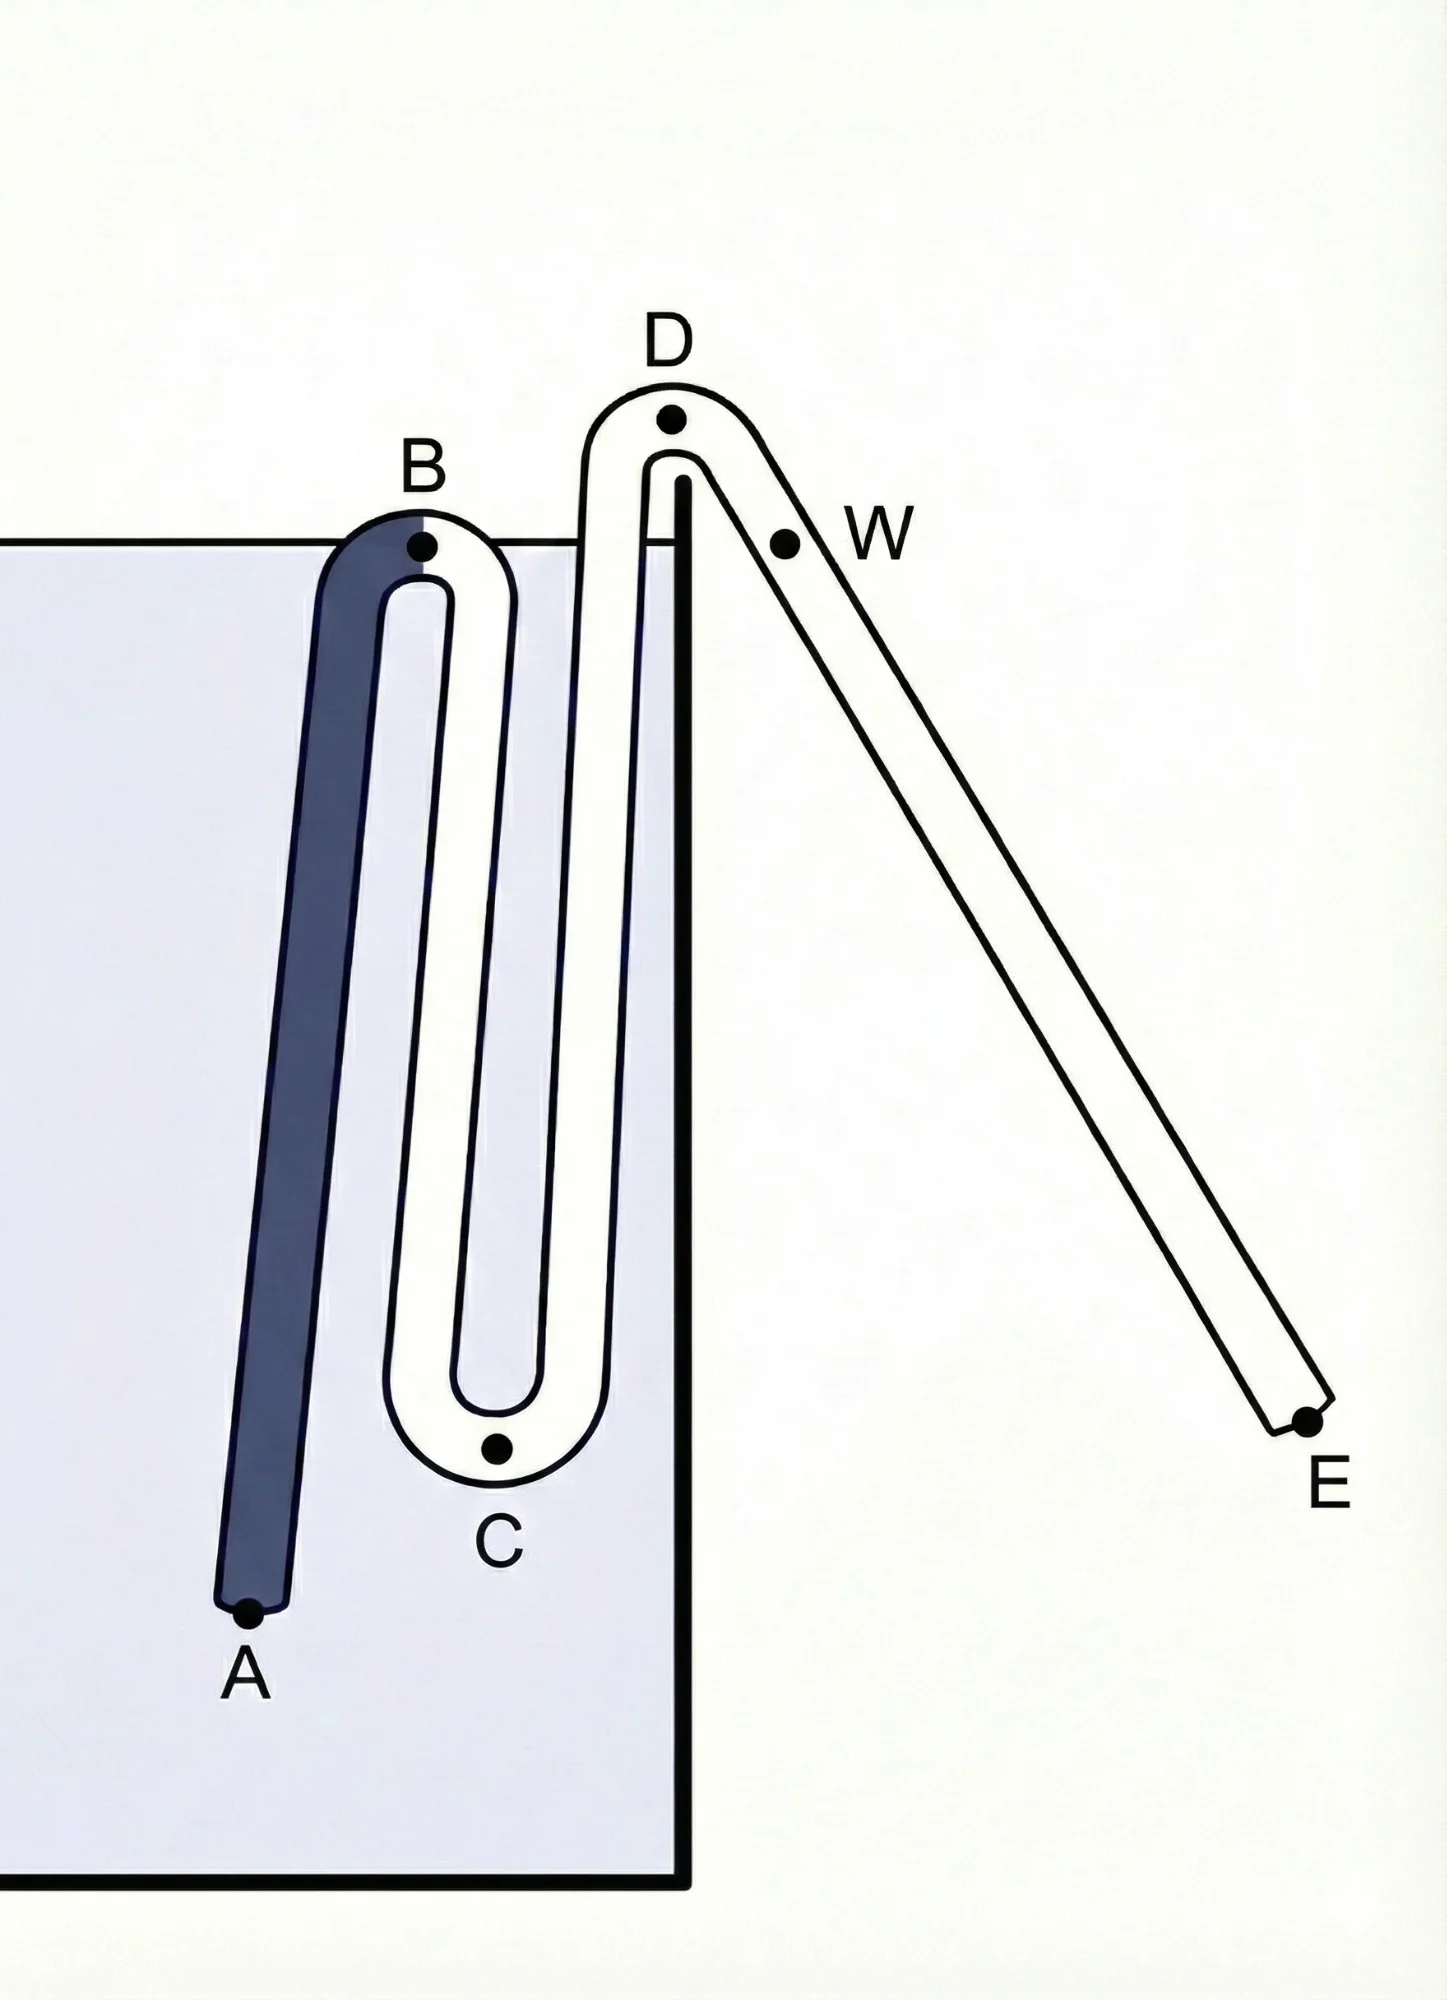
\includegraphics[width=0.6\textwidth]{siphon_schematic.png}
  \caption{Σχηματικό της γεωμετρίας του αυτοεκκινούμενου σιφώνα. Η στάθμη νερού του δοχείου $h_c^{(0)}$ βρίσκεται μεταξύ της πρώτης κορυφής $B$ και της κύριας κορυφής $D$. Ο κόμβος $A$ είναι η είσοδος· το τμήμα $A \to B$ γεμίζει υδροστατικά. Η πτώση $B \to C$ δημιουργεί ορμή. Η ανάβαση $C \to D$ περνά πάνω από τη στάθμη. Το σημείο $W$ στο τμήμα $D \to E$ σημειώνει την τελευταία τομή με τη στάθμη.}
  \label{fig:schematic}
\end{figure}

% --- FIGURE 2: Centreline profile h(L) ---
\begin{figure}[H]
  \centering
  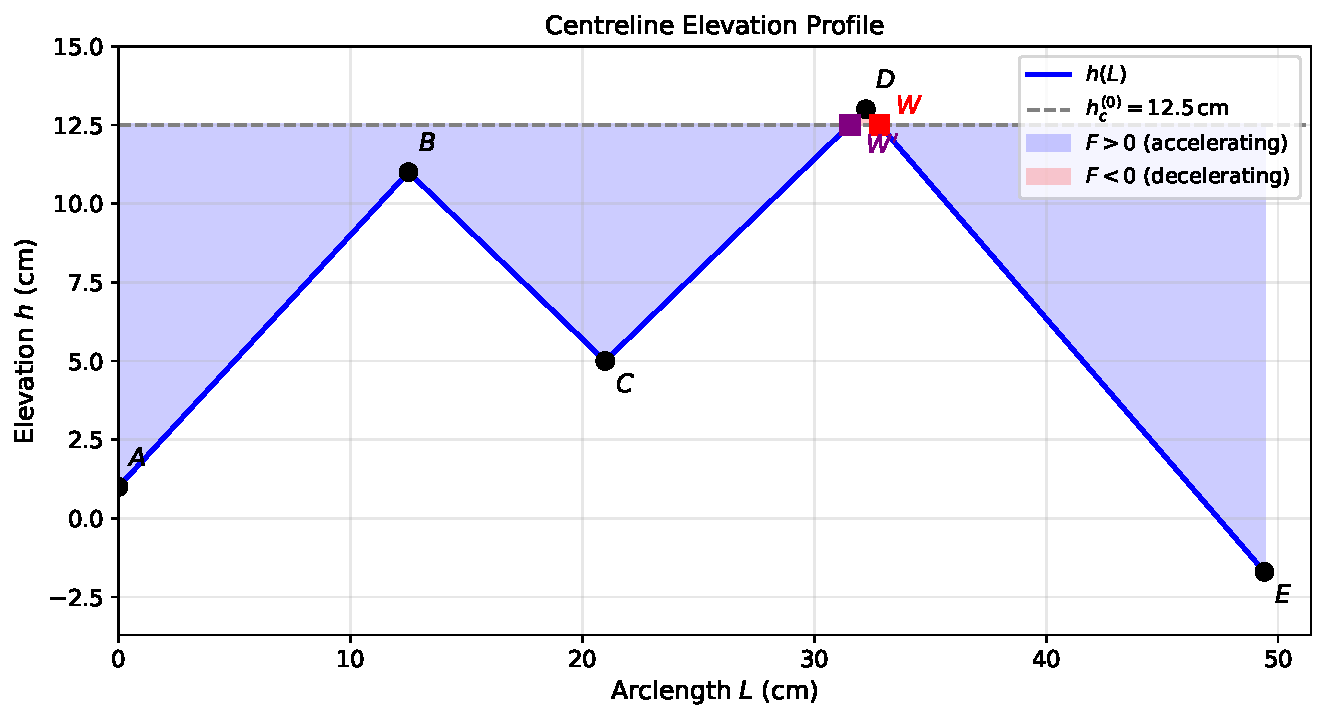
\includegraphics[width=0.9\textwidth]{figure2_centreline.pdf}
  \caption{Ύψος κεντρογραμμής $h(L)$ ως συνάρτηση του μήκους τόξου για το παράδειγμα αναφοράς. Η διακεκομμένη γραμμή δείχνει $h_c^{(0)} = 12.5$\,cm. Αφού φύγει από το $B$, το μέτωπο τέμνει αυτή τη στάθμη δύο φορές: μία ανερχόμενο (στο $W'$ στο $C \to D$) και μία κατερχόμενο (στο $W$ στο $D \to E$). Μπλε σκίαση: θετική κινητήρια δύναμη. Κόκκινη σκίαση: αρνητική κινητήρια δύναμη.}
  \label{fig:centreline}
\end{figure}

% ══════════════════════════════════════════════════════════════════════════════
%  SECTION 3: FRICTIONLESS MODEL
% ══════════════════════════════════════════════════════════════════════════════
\section{Το Μοντέλο χωρίς Τριβές: Επιδράσεις Γεωμετρίας}
\label{sec:frictionless}

Ξεκινάμε με δύο εξιδανικευτικές παραδοχές:
\begin{enumerate}[nosep,leftmargin=2em]
  \item \textbf{Χωρίς τριβές}: Αγνοούνται οι ιξώδεις απώλειες.
  \item \textbf{Χωρίς πτώση στάθμης}: Η στάθμη του δοχείου παραμένει σταθερή στο $h_c^{(0)}$.
\end{enumerate}

Αυτές οι παραδοχές απομονώνουν την επίδραση της γεωμετρίας. Οποιαδήποτε γεωμετρία αποτυγχάνει εδώ θα αποτύχει σίγουρα και στην πραγματικότητα.

\subsection{Η κινητήρια δύναμη}

Θεωρούμε το νερό μέσα στον σωλήνα ως βύσμα που εκτείνεται από την είσοδο μέχρι το μέτωπο στη θέση $L$. Οι δυνάμεις στο βύσμα είναι:

\paragraph{Πίεση στην είσοδο.} Η είσοδος σε ύψος $h_0$ βρίσκεται σε βάθος $h_c - h_0$ κάτω από την επιφάνεια. Η υδροστατική πίεση ωθεί το βύσμα προς τα εμπρός:
\[
  F_{\text{in}} = [p_{\text{atm}} + \rho g(h_c - h_0)] A.
\]

\paragraph{Πίεση στο μέτωπο.} Το μέτωπο επικοινωνεί με την ατμοσφαιρική πίεση στο άδειο τμήμα του σωλήνα μπροστά του:
\[
  F_{\text{front}} = p_{\text{atm}} A.
\]

\paragraph{Βαρύτητα κατά μήκος του βύσματος.} Ολοκληρώνοντας τη βαρύτητα κατά μήκος του βύσματος από την είσοδο (ύψος $h_0$) μέχρι το μέτωπο (ύψος $h(L)$):
\[
  F_{\text{gravity}} = -\rho g A [h(L) - h_0].
\]

Η ολική κινητήρια δύναμη είναι:
\begin{align}
  F &= F_{\text{in}} - F_{\text{front}} + F_{\text{gravity}} \notag \\
     &= \rho g A (h_c - h_0) - \rho g A [h(L) - h_0] \notag \\
     &= \rho g A [h_c - h(L)].
  \label{eq:driving-force}
\end{align}

Το ύψος της εισόδου απαλείφεται. Το αποτέλεσμα εξαρτάται μόνο από τη διαφορά υψομέτρου μεταξύ επιφάνειας δοχείου και μετώπου:
\begin{equation}
  \boxed{F = \rho g A [h_c - h(L)]}
  \label{eq:driving-force-boxed}
\end{equation}

\paragraph{Πρόσημο της κινητήριας δύναμης.}
\begin{itemize}[nosep,leftmargin=2em]
  \item $h(L) < h_c$: $F > 0$, το βύσμα επιταχύνεται και κερδίζει κινητική ενέργεια.
  \item $h(L) > h_c$: $F < 0$, το βύσμα επιβραδύνεται και χάνει κινητική ενέργεια.
  \item $h(L) = h_c$: $F = 0$, το βύσμα κινείται με αδράνεια.
\end{itemize}

\paragraph{Επιτάχυνση.} Ο δεύτερος νόμος του Νεύτωνα με μεταβαλλόμενη μάζα $m = \rho A L$:
\begin{equation}
  a = \frac{F}{\rho A L} = \frac{g[h_c - h(L)]}{L}.
  \label{eq:acceleration}
\end{equation}

Ακόμη κι όταν η δύναμη είναι μεγάλη (π.χ. στο χαμηλό σημείο $C$ όπου $h_c - h(L) = 15$\,cm), η επιτάχυνση μειώνεται λόγω του αυξανόμενου μήκους του βύσματος $L$.

\subsection{Το ενεργειακό ολοκλήρωμα}

Χρησιμοποιώντας $\ddot{L} = v \, dv/dL$ και την εξίσωση κίνησης $L \ddot{L} = g[h_c^{(0)} - h(L)]$:
\begin{equation}
  v \frac{dv}{dL} = \frac{g}{L}[h_c^{(0)} - h(L)].
  \label{eq:v-dv-dL}
\end{equation}

Ολοκληρώνοντας από $L = S_1$ (όπου $v = 0$) έως ένα γενικό $L$:
\[
  \frac{1}{2}v^2 = g \int_{S_1}^{L} \frac{h_c^{(0)} - h(r)}{r} \, dr.
\]

Ορίζουμε το \emph{ενεργειακό ολοκλήρωμα}:
\begin{equation}
  \boxed{I(L) = \int_{S_1}^{L} \frac{h_c^{(0)} - h(r)}{r} \, dr}
  \label{eq:energy-integral}
\end{equation}

Τότε:
\begin{equation}
  v(L) = \sqrt{2 g I(L)}, \qquad \text{provided } I(L) > 0.
  \label{eq:v-from-I}
\end{equation}

Το ολοκλήρωμα έχει δύο παράγοντες:
\begin{itemize}[nosep,leftmargin=2em]
  \item $h_c^{(0)} - h(r)$: το κινητήριο ύψος στη θέση $r$. Θετικό κάτω από τη στάθμη, αρνητικό πάνω από αυτή.
  \item $1/r$: η στάθμιση λόγω μεταβαλλόμενης μάζας. Οι πρώιμες συνεισφορές (μικρό βύσμα) έχουν μεγαλύτερο βάρος.
\end{itemize}

Το βύσμα σταματά όταν $I(L) = 0$.

\subsection{Κριτήριο προπλήρωσης}

Η προπλήρωση επιτυγχάνει αν το βύσμα φτάσει στο σημείο $W$ με θετική ταχύτητα:
\begin{equation}
  \boxed{I(S_W) > 0 \quad \Longleftrightarrow \quad \text{η προπλήρωση επιτυγχάνει (χωρίς τριβές)}}
  \label{eq:priming-criterion}
\end{equation}

Πέρα από το $W$, το μέτωπο βρίσκεται μόνιμα κάτω από τη στάθμη, οπότε το $I(L)$ μόνο αυξάνεται.

\subsection{Υπολογισμός για κατά τμήματα γραμμική γεωμετρία}

Σε ένα τμήμα όπου $h(r) = c + sr$, η συνεισφορά του διαστήματος $[a, b]$ είναι:
\begin{equation}
  \Phi(a, b; c, s) = (h_c^{(0)} - c) \ln\frac{b}{a} - s(b - a).
  \label{eq:Phi-def}
\end{equation}

Για να υπολογίσουμε το $I(L)$ όταν το $L$ βρίσκεται στο τμήμα $k$:
\begin{equation}
  I(L) = \sum_{j=2}^{k-1} \Phi(S_{j-1}, S_j; c_j, s_j) + \Phi(S_{k-1}, L; c_k, s_k).
  \label{eq:I-piecewise}
\end{equation}

\subsection{Παράδειγμα αναφοράς}

Ο υπολογισμός του $I(S_W)$ απαιτεί συνεισφορές από τα τμήματα 2, 3 και ένα μέρος του 4.

\paragraph{Τμήμα 2 ($B \to C$), διάστημα $[12.50, 20.99]$\,cm:}
\[
  \Phi_2 = (12.5 - 19.84)\ln\frac{20.99}{12.50} - (-0.707)(8.49) = -3.80 + 6.00 = +2.20\,\text{cm}.
\]

\paragraph{Τμήμα 3 ($C \to D$), διάστημα $[20.99, 32.23]$\,cm:}
\[
  \Phi_3 = (12.5 - (-9.93))\ln\frac{32.23}{20.99} - (0.712)(11.24) = 9.62 - 8.00 = +1.62\,\text{cm}.
\]

\paragraph{Τμήμα 4 ($D \to W$), διάστημα $[32.23, 32.81]$\,cm:}
\[
  \Phi_4 = (12.5 - 40.57)\ln\frac{32.81}{32.23} - (-0.855)(0.58) = -0.50 + 0.50 = -0.005\,\text{cm}.
\]

\paragraph{Σύνολο:}
\begin{equation}
  I(S_W) = 2.20 + 1.62 - 0.005 = 3.82\,\text{cm} > 0.
  \label{eq:I-SW-value}
\end{equation}

Το κριτήριο ικανοποιείται. Η ταχύτητα χωρίς τριβές στο $W$:
\[
  v_W = \sqrt{2 \times 981 \times 3.82} = 86.5\,\text{cm/s} = 0.865\,\text{m/s}.
\]

\subsection{Σχεδιαστικά συμπεράσματα}

Το ενεργειακό ολοκλήρωμα αποκαλύπτει πώς η γεωμετρία ελέγχει την προπλήρωση:

\begin{itemize}[nosep,leftmargin=2em]
  \item \textbf{Οι απότομες πτώσεις νωρίς είναι οι πιο αποτελεσματικές.} Η στάθμιση $\ln(b/a)$ σημαίνει ότι τα πρώιμα τμήματα (μικρό $r$) συνεισφέρουν περισσότερο ανά μονάδα μήκους. Η πτώση $B \to C$ συμβαίνει για $L \in [17, 31]$\,cm όταν το βύσμα είναι ακόμη μικρό.

  \item \textbf{Μέρος της ανόδου είναι «δωρεάν».} Το τμήμα 3 συνεισφέρει θετικά, παρότι είναι ανηφορικό, επειδή ένα μέρος του παραμένει κάτω από τη στάθμη.

  \item \textbf{Η περιοχή πάνω από τη στάθμη κοστίζει ενέργεια.} Η συνεισφορά $\Phi_4 = -0.16$\,cm είναι αρνητική. Κρατήστε την κορυφή χαμηλά και την κάθοδο απότομη.

  \item \textbf{Προέλεγχος χωρίς προσομοίωση.} Το κριτήριο $I(S_W) > 0$ υπολογίζεται αναλυτικά. Γεωμετρίες που αποτυγχάνουν μπορούν να απορριφθούν άμεσα.
\end{itemize}

% --- FIGURE 3: Driving force and acceleration ---
\begin{figure}[H]
  \centering
  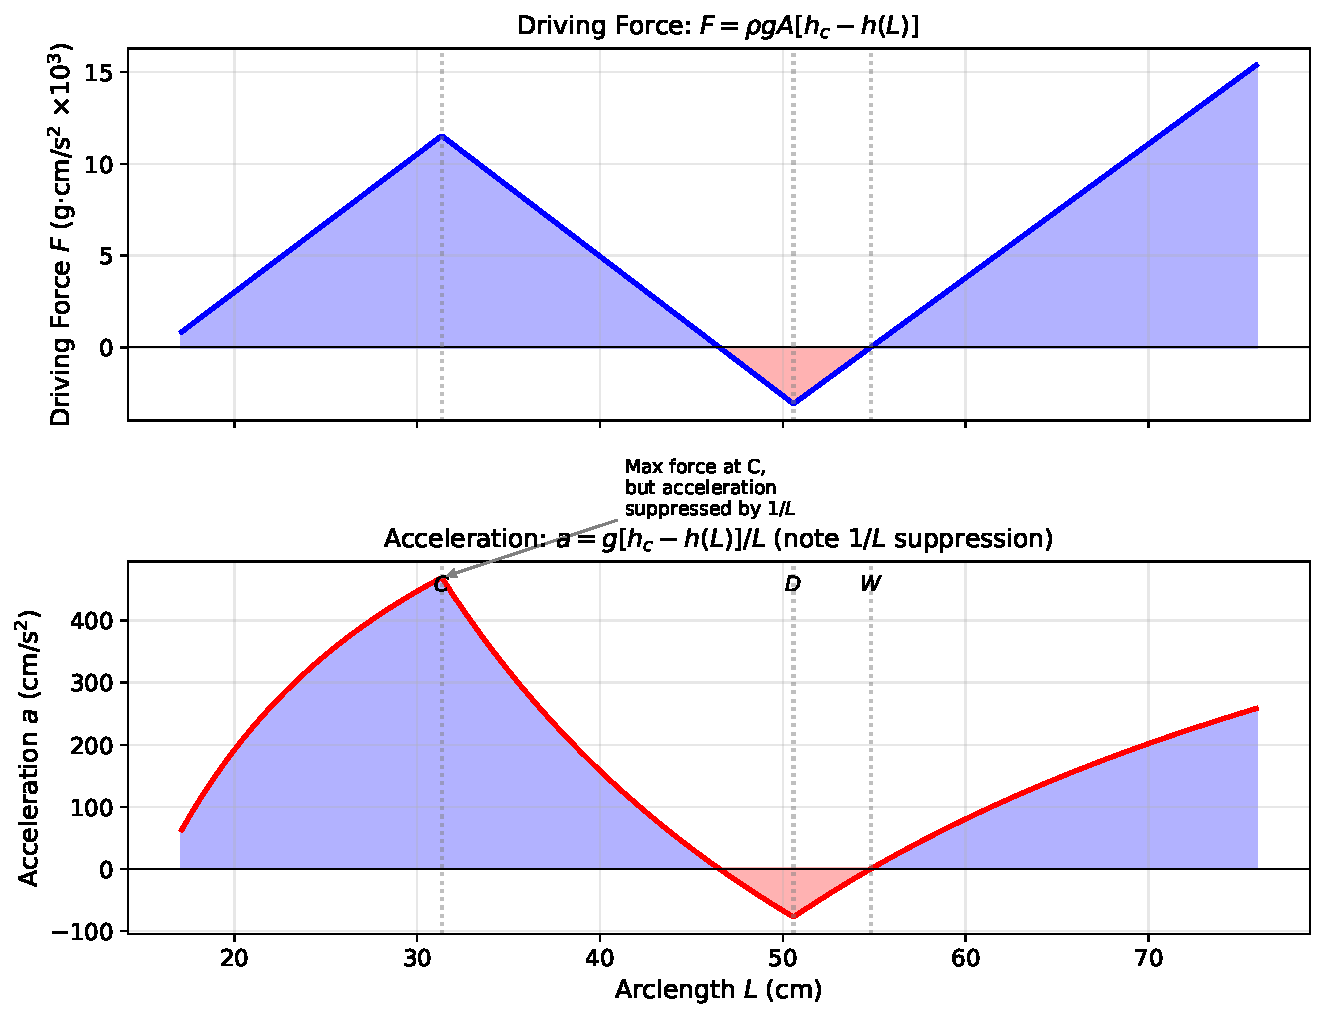
\includegraphics[width=0.9\textwidth]{figure3_force_acceleration.pdf}
  \caption{Πάνω: Κινητήρια δύναμη $F(L) = \rho g A[h_c^{(0)} - h(L)]$ ως συνάρτηση του μήκους τόξου. Η δύναμη αλλάζει πρόσημο στις τομές με τη στάθμη. Κάτω: Επιτάχυνση $a(L) = g[h_c^{(0)} - h(L)]/L$. Ακόμη και στο σημείο $C$ όπου η δύναμη είναι μέγιστη, η επιτάχυνση μετριάζεται από το μήκος του βύσματος $L$. Ο παράγοντας $1/L$ προκαλεί μείωση της επιτάχυνσης καθώς το βύσμα μεγαλώνει.}
  \label{fig:force-acceleration}
\end{figure}

% --- FIGURE 4: Energy integral I(L) ---
\begin{figure}[H]
  \centering
  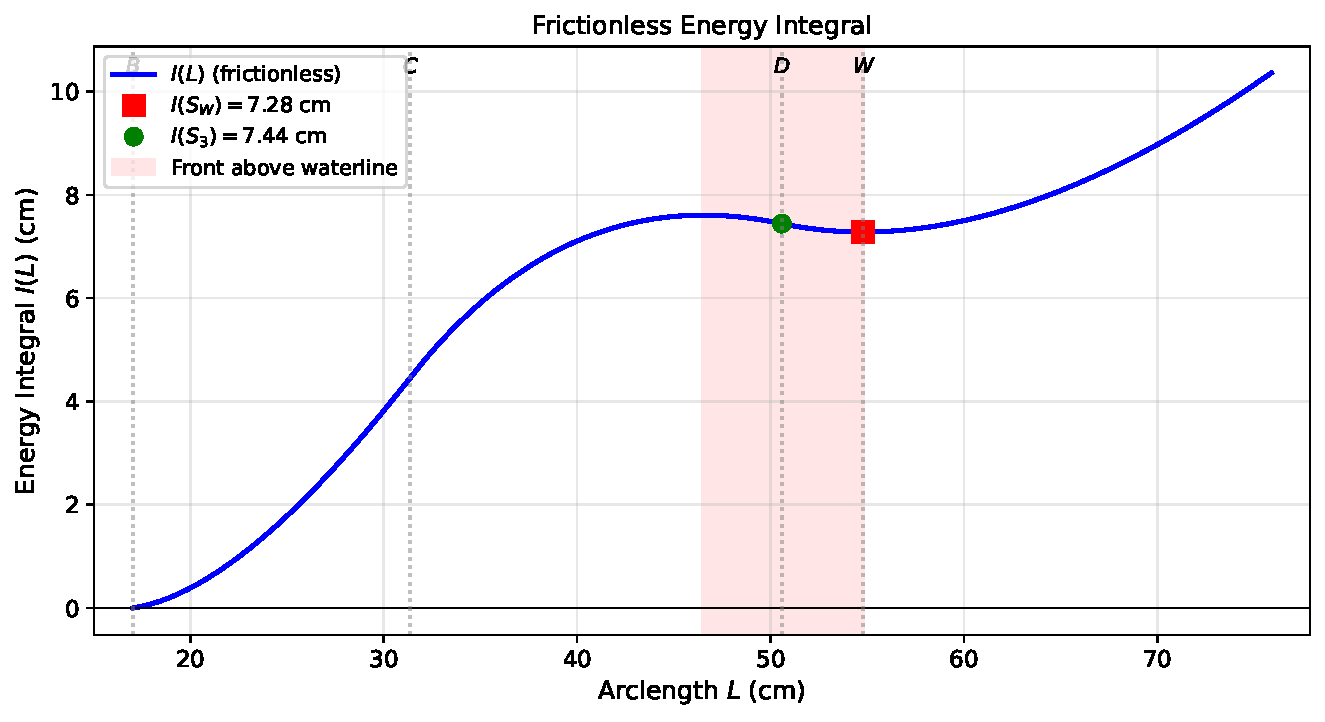
\includegraphics[width=0.9\textwidth]{figure4_energy_integral.pdf}
  \caption{Ενεργειακό ολοκλήρωμα $I(L)$ ως συνάρτηση του μήκους τόξου (χωρίς τριβές, χωρίς πτώση στάθμης). Το ολοκλήρωμα αυξάνει κατά την πτώση $B \to C$, συνεχίζει να αυξάνει στην αρχή της ανόδου (όπου $h < h_c^{(0)}$), και στη συνέχεια μειώνεται ελαφρά όσο το μέτωπο βρίσκεται πάνω από τη στάθμη (μεταξύ $W'$ και $W$). Στο σημείο $W$, $I(S_W) = 3.82$\,cm $> 0$: η προπλήρωση επιτυγχάνει.}
  \label{fig:energy-integral}
\end{figure}

% ══════════════════════════════════════════════════════════════════════════════
%  SECTION 4: DRAWDOWN
% ══════════════════════════════════════════════════════════════════════════════
\section{Προσθήκη Πτώσης Στάθμης Δοχείου: Επιδράσεις Μεγέθους Συστήματος}
\label{sec:drawdown}

Καθώς το νερό εισέρχεται στον σωλήνα, η στάθμη στο δοχείο πέφτει. Αυτή η \emph{πτώση στάθμης} μειώνει την κινητήρια δύναμη.

\subsection{Η σχέση πτώσης στάθμης}

Διατήρηση όγκου: το νερό που εισέρχεται στον σωλήνα ισούται με το νερό που χάνει το δοχείο.
\[
  A(L - S_1) = A_0[h_c^{(0)} - h_c(L)].
\]

Λύνοντας:
\begin{equation}
  \boxed{h_c(L) = h_c^{(0)} - \frac{A}{A_0}(L - S_1)}
  \label{eq:drawdown}
\end{equation}

Η στάθμη του δοχείου μειώνεται γραμμικά με τη θέση του βύσματος, με ρυθμό $A/A_0$.

\subsection{Τροποποιημένο ενεργειακό ολοκλήρωμα}

Με πτώση στάθμης, το κινητήριο ύψος γίνεται $h_c(L) - h(L)$ αντί για $h_c^{(0)} - h(L)$. Το ενεργειακό ολοκλήρωμα γίνεται:
\begin{equation}
  I_{\text{dd}}(L) = \int_{S_1}^{L} \frac{h_c^{(0)} - \frac{A}{A_0}(r - S_1) - h(r)}{r} \, dr.
  \label{eq:I-dd-def}
\end{equation}

Αυτό γράφεται ως:
\begin{equation}
  I_{\text{dd}}(L) = I(L) - \frac{A}{A_0} \int_{S_1}^{L} \frac{r - S_1}{r} \, dr.
  \label{eq:I-dd-split}
\end{equation}

Το ολοκλήρωμα «ποινή» της πτώσης στάθμης υπολογίζεται ως:
\begin{equation}
  \int_{S_1}^{L} \frac{r - S_1}{r} \, dr = (L - S_1) - S_1 \ln\frac{L}{S_1}.
  \label{eq:drawdown-penalty}
\end{equation}

\subsection{Παράδειγμα αναφοράς}

Για το παράδειγμα αναφοράς με $A/A_0 = 5.77\times 10^{-4}$, στο $L = S_W = 32.81$\,cm:
\[
  (32.81 - 12.50) - 12.50 \ln\frac{32.81}{12.50} = 20.31 - 12.06 = 8.25\,\text{cm}.
\]

Ποινή πτώσης στάθμης:
\[
  \frac{A}{A_0} \times 8.25 = (5.77\times 10^{-4}) \times 8.25 = 0.0048\,\text{cm}.
\]

Τροποποιημένο ολοκλήρωμα:
\begin{equation}
  I_{\text{dd}}(S_W) = 3.82 - 0.005 = 3.81\,\text{cm} > 0.
  \label{eq:I-dd-value}
\end{equation}

Η πτώση στάθμης μειώνει το περιθώριο μόνο κατά $\sim 0.1\%$ για αυτό το μεγάλο δοχείο.

\subsection{Πότε έχει σημασία η πτώση στάθμης}

Η συνολική πτώση στάθμης όταν το μέτωπο φτάσει στην έξοδο:
\[
  \Delta h_c = \frac{A}{A_0}(S_4 - S_1) = (5.77\times 10^{-4}) \times 36.91 = 0.021\,\text{cm}.
\]

Για ένα μικρότερο δοχείο με $A_0 = 20\,\text{cm}^2$ (λόγος εμβαδών $A/A_0 \approx 0.0098$):
\[
  \Delta h_c \approx 0.0098 \times 36.91 = 0.36\,\text{cm}.
\]

Αυτό θα μείωνε το αρχικό κινητήριο ύψος $h_c^{(0)} - h_1 = 1.5$\,cm στον κόμβο $B$, κάτι που μπορεί να προκαλέσει αποτυχία σε οριακές γεωμετρίες.

\paragraph{Κύρια παράμετρος: $A/A_0$.} Όταν $A/A_0 \ll 0.01$, η πτώση στάθμης είναι αμελητέα. Όταν $A/A_0 \gtrsim 0.01$, η πτώση στάθμης πρέπει να λαμβάνεται υπόψη.

% --- FIGURE 5: Container level h_c(L) ---
\begin{figure}[H]
  \centering
  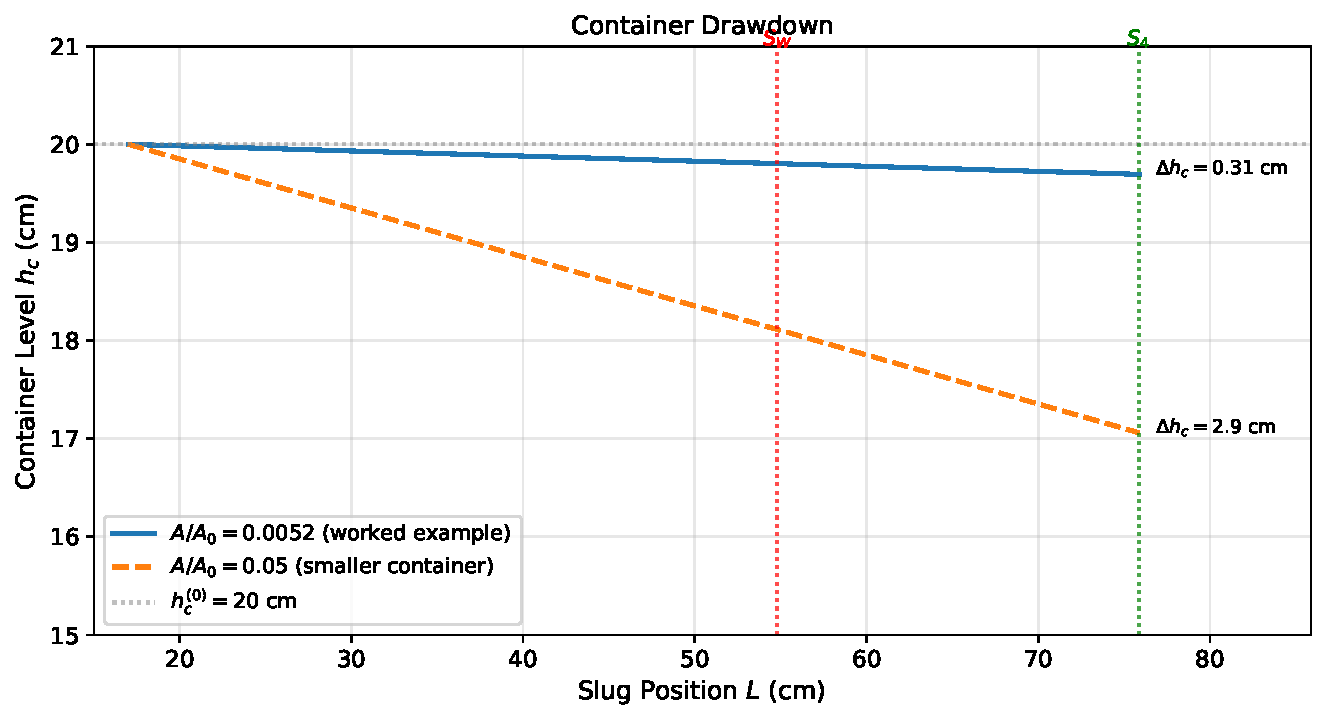
\includegraphics[width=0.9\textwidth]{figure5_drawdown.pdf}
  \caption{Στάθμη δοχείου $h_c(L)$ ως συνάρτηση της θέσης του βύσματος για δύο λόγους εμβαδών. Συνεχής γραμμή: $A/A_0 = 5.77\times 10^{-4}$ (πείραμα). Διακεκομμένη: $A/A_0 = 0.05$ (μικρότερο δοχείο). Κατακόρυφες διάστικτες γραμμές δείχνουν $S_W$ και $S_4$. Για το πείραμα, η πτώση στάθμης είναι αμελητέα ($\Delta h_c \approx 0.02$\,cm μέχρι την έξοδο).}
  \label{fig:drawdown}
\end{figure}

% ══════════════════════════════════════════════════════════════════════════════
%  SECTION 5: FRICTION
% ══════════════════════════════════════════════════════════════════════════════
\section{Προσθήκη Τριβών: Επιδράσεις Σωλήνα}
\label{sec:friction}

Η ιξώδης τριβή διαχέει κινητική ενέργεια. Αρχικά αναπτύσσουμε ένα μοντέλο σταθερού συντελεστή τριβής που διατηρεί την αναλυτική αντιμετώπιση, και έπειτα συζητάμε την τριβή που εξαρτάται από την ταχύτητα για την πλήρη δυναμική.

\subsection{Απώλειες φορτίου λόγω τριβών}

Η εξίσωση Darcy--Weisbach δίνει την απώλεια φορτίου κατά μήκος σωλήνα μήκους $L$:
\begin{equation}
  h_f = f \frac{L}{D} \frac{v^2}{2g},
  \label{eq:darcy-weisbach}
\end{equation}
όπου $f$ είναι ο συντελεστής τριβής Darcy.

Οι τοπικές απώλειες στις καμπές προσθέτουν:
\begin{equation}
  h_{\text{minor}} = \sum K \frac{v^2}{2g}.
  \label{eq:minor-loss}
\end{equation}

Συνολική απώλεια φορτίου:
\begin{equation}
  h_{\text{loss}} = \left(f\frac{L}{D} + \sum K\right) \frac{v^2}{2g}.
  \label{eq:total-loss}
\end{equation}

\subsection{Η προσέγγιση σταθερού συντελεστή τριβής}

Ο συντελεστής τριβής $f$ εξαρτάται από τον αριθμό Reynolds $\text{Re} = vD/\nu$, ο οποίος μεταβάλλεται κατά την πλήρωση. Ωστόσο, η υπόθεση ότι το $f$ είναι σταθερό επιτρέπει αναλυτική λύση.

Αυτή η προσέγγιση είναι ακριβής στο καθεστώς πλήρως τραχείας ροής, όπου το $f$ εξαρτάται μόνο από $\varepsilon/D$:
\begin{equation}
  \frac{1}{\sqrt{f}} = -2\log\left(\frac{\varepsilon/D}{3.7}\right).
  \label{eq:fully-rough}
\end{equation}

Πιο γενικά, η επιλογή μιας αντιπροσωπευτικής τιμής $f_0$ από το αναμενόμενο εύρος Reynolds εισάγει σφάλματα συγκρίσιμα με άλλες αβεβαιότητες του μοντέλου. Για το παράδειγμα αναφοράς, χρησιμοποιούμε $f_0 \approx 0.078$, επιλεγμένο από το εύρος Reynolds της φάσης πλήρωσης, αφού προσαρμόσουμε το $\sum K$ στην πειραματική καμπύλη $v(L)$.

\subsection{Ενεργειακό ολοκλήρωμα με διόρθωση τριβών}

Με σταθερή τριβή και χωρίς πτώση στάθμης, η εξίσωση κίνησης γίνεται:
\[
  v \frac{dv}{dL} + \left(\frac{f_0}{D} + \frac{\sum K}{L}\right) \frac{v^2}{2} = \frac{g}{L}[h_c^{(0)} - h(L)].
\]

Θέτοντας $u = v^2/2$ προκύπτει μια γραμμική Δ.Ε. πρώτης τάξης:
\begin{equation}
  \frac{du}{dL} + \left(\frac{f_0}{D} + \frac{\sum K}{L}\right) u = \frac{g}{L}[h_c^{(0)} - h(L)].
  \label{eq:u-ODE}
\end{equation}

Ο ολοκληρωτικός παράγοντας είναι:
\begin{equation}
  \mu(L) = \left(\frac{L}{S_1}\right)^{\sum K} \exp\left(\frac{f_0(L - S_1)}{D}\right).
  \label{eq:integrating-factor}
\end{equation}

Με $u(S_1) = 0$, η λύση ορίζει το \emph{ενεργειακό ολοκλήρωμα με διόρθωση τριβών}:
\begin{equation}
  \boxed{I_f(L) = \frac{1}{\mu(L)} \int_{S_1}^{L} \mu(r) \frac{h_c^{(0)} - h(r)}{r} \, dr}
  \label{eq:I-f-def}
\end{equation}
με $v(L) = \sqrt{2gI_f(L)}$.

\subsection{Φυσική ερμηνεία}

Στο ολοκλήρωμα χωρίς τριβές, κάθε θέση $r$ συνεισφέρει με βάρος $1/r$. Με τριβές, το αποτελεσματικό βάρος γίνεται:
\[
  \frac{\mu(r)}{\mu(L)} \cdot \frac{1}{r} = \frac{1}{r}\left(\frac{r}{L}\right)^{\sum K} \exp\left(-\frac{f_0(L-r)}{D}\right).
\]

Ο εκθετικός παράγοντας \emph{απομειώνει} τις συνεισφορές από πιο πρώιμες θέσεις: η ενέργεια που «αποθηκεύεται» νωρίς έχει μεγαλύτερη απόσταση να διανύσει και υφίσταται μεγαλύτερη διάχυση. Ο προπαράγοντας $1/\mu(L)$ αντανακλά τη σωρευτική διάχυση σε όλη τη διαδρομή.

Εφόσον $\mu(r)/\mu(L) < 1$ για $r < L$, ισχύει πάντα $I_f(L) < I(L)$.

\subsection{Παράδειγμα αναφοράς}

Για $f_0 \approx 0.078$, $\sum K = 14.4$, $D = 0.5$\,cm, στο $L = S_W = 32.81$\,cm:
\[
  \mu(S_W) = \left(\frac{32.81}{12.50}\right)^{14.4} \exp\left(\frac{0.078 \times 20.31}{0.5}\right) \approx (2.62)^{14.4} \times e^{3.16} \approx 2.5\times 10^{7}.
\]

Αριθμητική αξιολόγηση δίνει:
\begin{equation}
  I_f(S_W) \approx 0.020\,\text{cm} > 0.
  \label{eq:I-f-value}
\end{equation}

Σε σύγκριση με $I(S_W) = 3.82$\,cm, το μοντέλο σταθερής τριβής μειώνει τη διαθέσιμη ενέργεια κατά $\sim 99.5\%$. Η ταχύτητα στο $W$:
\[
  v_W = \sqrt{2 \times 981 \times 0.020} \approx 6.3\,\text{cm/s} \approx 0.063\,\text{m/s}.
\]

Το κριτήριο προπλήρωσης ικανοποιείται οριακά στο συντηρητικό μοντέλο σταθερής τριβής. Αυτό αντανακλά την πειραματική πραγματικότητα για σίφωνα μικρής διαμέτρου: οι αποτελεσματικές τοπικές απώλειες (καμπές, είσοδος/έξοδος και μη μοντελοποιημένη διάχυση) μπορούν να κυριαρχήσουν στο ενεργειακό ισοζύγιο, αφήνοντας μικρό περιθώριο κοντά στο όριο.

\subsection{Πότε έχουν σημασία οι τριβές}

Οι βασικές παράμετροι είναι $\varepsilon/D$ (σχετική τραχύτητα) και $\sum K$ (απώλειες καμπών).

Για το παράδειγμα αναφοράς, η μετρημένη μέγιστη ταχύτητα πλήρωσης είναι $v \approx 0.36$\,m/s. Με $D = 5$\,mm και $\nu = 10^{-6}\,\text{m}^2/\text{s}$:
\[
  \text{Re} \approx \frac{0.36 \times 0.005}{10^{-6}} \approx 1800,
\]
οπότε η ροή είναι κυρίως στρωτή και $f \approx 64/\text{Re} \approx 0.036$· η τραχύτητα έχει μικρή επίδραση σε αυτό το καθεστώς.

Απώλεια φορτίου από κατανεμημένες τριβές σε όλο τον σωλήνα ($L_{\max} = 0.494$\,m):
\[
  h_f \approx 0.036 \times \frac{0.494}{0.005} \times \frac{0.36^2}{2 \times 9.81} \approx 0.023\,\text{m} \approx 2.3\,\text{cm}.
\]

Τοπικές απώλειες (αποτελεσματικό προσαρμοσμένο $\sum K \approx 14.4$):
\[
  h_{\text{minor}} \approx 14.4 \times \frac{0.36^2}{2 \times 9.81} \approx 0.095\,\text{m} \approx 9.5\,\text{cm}.
\]

Έτσι, ακόμη και για μέτριους αριθμούς Reynolds, οι τοπικές απώλειες μπορούν να κυριαρχήσουν στο ενεργειακό ισοζύγιο για σίφωνες μικρής διαμέτρου. Αυτό δικαιολογεί την αντιμετώπιση του $\sum K$ ως αποτελεσματικής παραμέτρου όταν οι λεπτομέρειες των καμπών και τα φαινόμενα εισόδου/εξόδου δεν μετρώνται.

% --- FIGURE 6: Friction factor f(Re) ---
\begin{figure}[H]
  \centering
  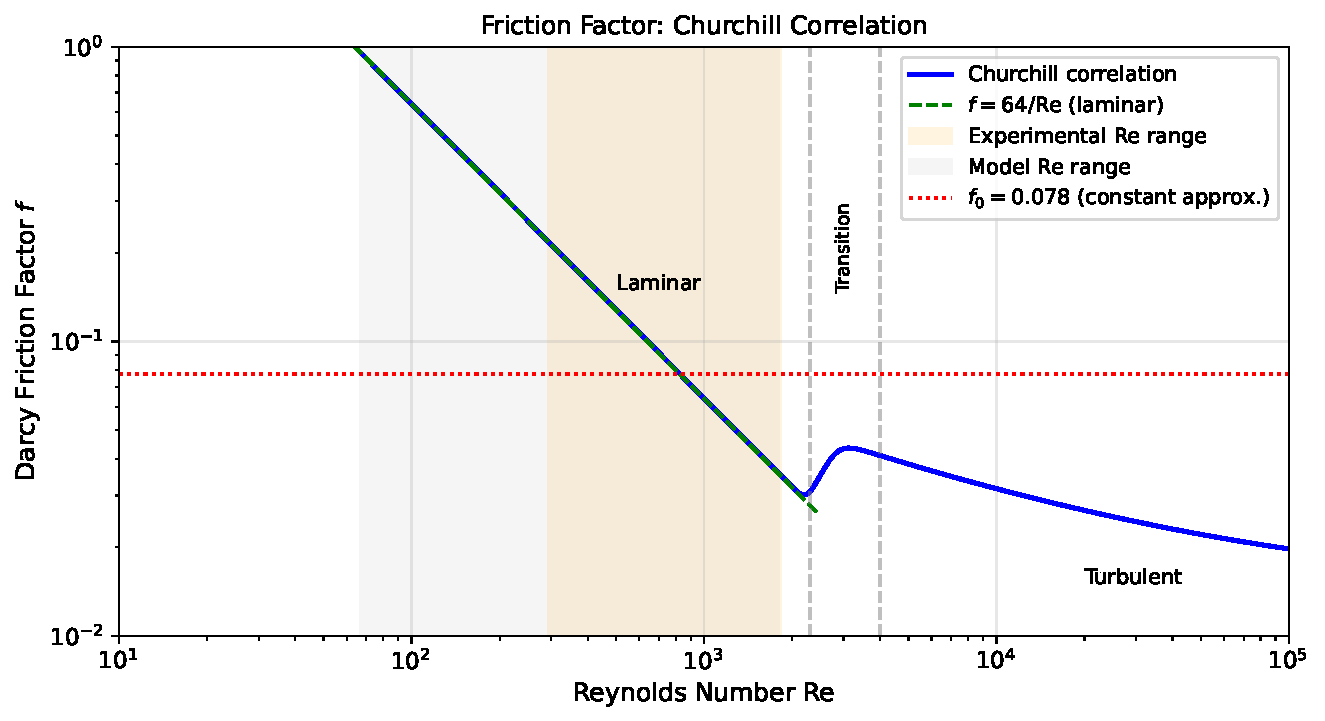
\includegraphics[width=0.9\textwidth]{figure6_friction.pdf}
  \caption{Συντελεστής τριβής $f$ ως συνάρτηση του αριθμού Reynolds από τη συσχέτιση Churchill. Διακρίνονται τρία καθεστώτα: στρωτό ($f = 64/\text{Re}$), μεταβατικό και τυρβώδες. Οι σκιασμένες ζώνες δείχνουν τα πειραματικά και μοντελικά εύρη Reynolds κατά την πλήρωση (και τα δύο κυρίως κάτω από $\text{Re} \approx 2000$). Η οριζόντια διακεκομμένη γραμμή δείχνει $f_0 \approx 0.078$, την προσέγγιση σταθερού συντελεστή τριβής.}
  \label{fig:friction}
\end{figure}

% ══════════════════════════════════════════════════════════════════════════════
%  SECTION 6: COMPARING THE THREE MODELS
% ══════════════════════════════════════════════════════════════════════════════
\section{Σύγκριση των Τριών Μοντέλων}
\label{sec:comparison}

Πλέον έχουμε τρία ενεργειακά ολοκληρώματα που σχηματίζουν μια ιεραρχία:
\begin{equation}
  I(L) \geq I_{\text{dd}}(L) \geq I_f(L).
  \label{eq:hierarchy}
\end{equation}

\subsection{Σύνοψη τιμών στο $S_W$}

\begin{center}
\renewcommand{\arraystretch}{1.3}
\begin{tabular}{lccc}
\toprule
Μοντέλο & Ολοκλήρωμα στο $S_W$ & Ταχύτητα στο $W$ & Κύρια παράμετρος \\
\midrule
Χωρίς τριβές & $I = 3.82$\,cm & 0.865\,m/s & Γεωμετρία \\
Με πτώση στάθμης & $I_{\text{dd}} = 3.81$\,cm & 0.86\,m/s & $A/A_0 = 5.77\times 10^{-4}$ \\
Με τριβές & $I_f \approx 0.020$\,cm & 0.063\,m/s & $\varepsilon/D$, $\sum K$ \\
\bottomrule
\end{tabular}
\end{center}

\subsection{Φυσική ερμηνεία}

\paragraph{Ολοκλήρωμα χωρίς τριβές $I(L)$:} Το άνω όριο. Αντιπροσωπεύει τη μέγιστη κινητική ενέργεια που μπορεί να προκύψει μόνο από τη γεωμετρία. Αν $I(S_W) \leq 0$, καμία μείωση τριβών δεν μπορεί να «σώσει» τη διάταξη.

\paragraph{Ολοκλήρωμα με πτώση στάθμης $I_{\text{dd}}(L)$:} Λαμβάνει υπόψη την πτώση της στάθμης στο δοχείο. Η μείωση $I - I_{\text{dd}}$ αυξάνει με το $A/A_0$ και με το μήκος του βύσματος. Για το παράδειγμα αναφοράς με μεγάλο δοχείο, η πτώση στάθμης μειώνει το περιθώριο μόνο κατά $\sim 0.1\%$.

\paragraph{Ολοκλήρωμα με τριβές $I_f(L)$:} Λαμβάνει υπόψη τη διάχυση ενέργειας. Για το παράδειγμα αναφοράς με αποτελεσματικό $\sum K \approx 14.4$, το ολοκλήρωμα σταθερής τριβής μειώνει τη διαθέσιμη ενέργεια κατά $\sim 99.5\%$. Αυτή η μεγάλη μείωση προκύπτει από τον παράγοντα $(L/S_1)^{\sum K}$ στον ολοκληρωτικό παράγοντα μαζί με την εκθετική απομείωση, οι οποίοι τιμωρούν έντονα την ενέργεια που «αποθηκεύεται» νωρίς κατά μήκος της διαδρομής. Το μοντέλο σταθερής τριβής είναι συντηρητικό: δίνει ένα κάτω όριο που, αν και απαισιόδοξο, εγγυάται προπλήρωση αν $I_f(S_W) > 0$.

\subsection{Συνέπειες για τον γεωμετρικό προέλεγχο}

Μια γεωμετρία με $I(S_W) = 3$\,cm περνά τον έλεγχο χωρίς τριβές αλλά μπορεί να έχει $I_f(S_W) < 0$ και να αποτύχει όταν συμπεριληφθούν τριβές. Για το παράδειγμα αναφοράς με αποτελεσματικό $\sum K \approx 14.4$, το μοντέλο σταθερής τριβής προβλέπει $I_f(S_W) \approx 0.020$\,cm---ένα μικρό αλλά θετικό περιθώριο. Αυτή η ευαισθησία στις τοπικές απώλειες υποδεικνύει:
\begin{itemize}[nosep,leftmargin=2em]
  \item \textbf{Η γεωμετρία των καμπών έχει μεγαλύτερη σημασία από την τραχύτητα.} Ο όρος $\sum K$ κυριαρχεί.
  \item \textbf{Πιο ομαλές καμπές βελτιώνουν δραματικά το περιθώριο.} Η μείωση του $\sum K$ αυξάνει σημαντικά το $I_f(S_W)$ και άρα το περιθώριο προπλήρωσης.
  \item \textbf{Το μοντέλο σταθερής τριβής είναι συντηρητικό.} Η πλήρης Δ.Ε. με τριβή που εξαρτάται από την ταχύτητα συνήθως προβλέπει καλύτερη απόδοση.
\end{itemize}

% --- FIGURE 7: Comparison of three integrals ---
\begin{figure}[H]
  \centering
  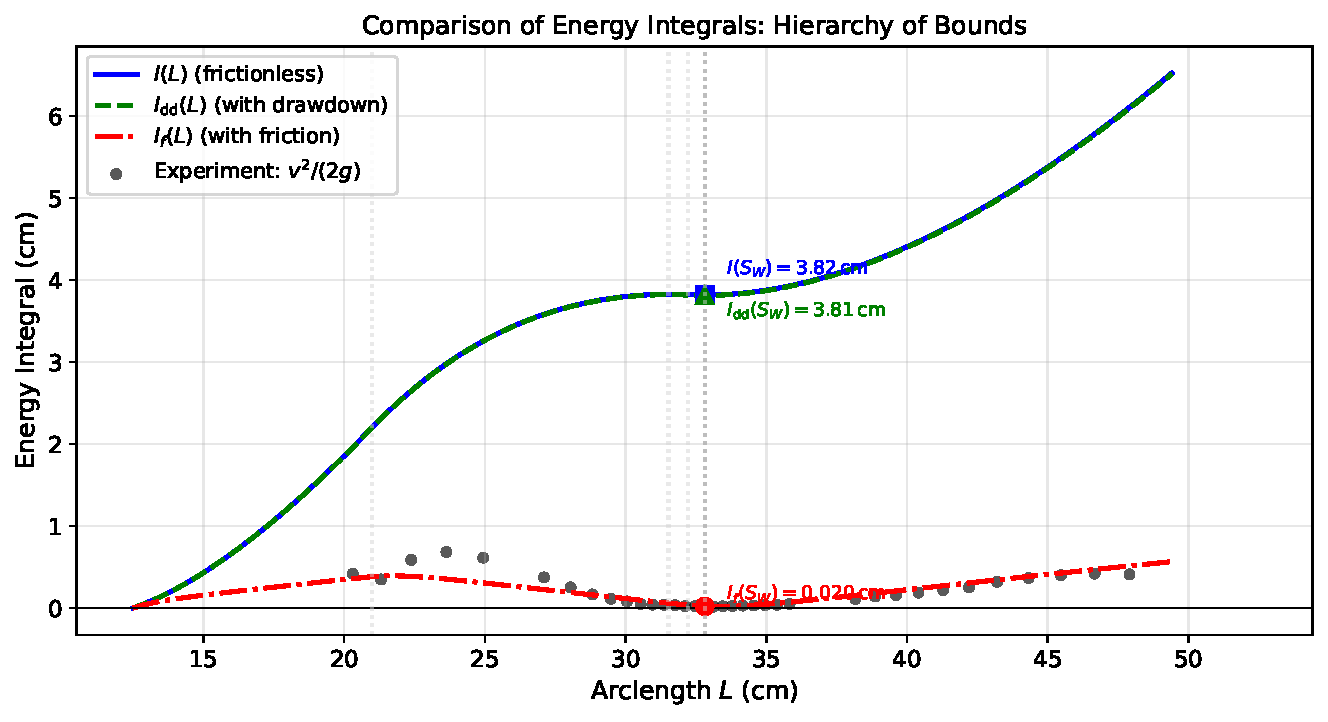
\includegraphics[width=0.9\textwidth]{figure7_comparison.pdf}
  \caption{Σύγκριση των ενεργειακών ολοκληρωμάτων $I(L)$, $I_{\text{dd}}(L)$ και $I_f(L)$ ως συνάρτηση του μήκους τόξου για το παράδειγμα αναφοράς. Το ολοκλήρωμα χωρίς τριβές (συνεχές) δίνει το άνω όριο. Η πτώση στάθμης (διακεκομμένο) το μειώνει ελάχιστα. Οι τριβές (διακεκομμένο-στιγμές) προκαλούν μεγάλη μείωση, ιδιαίτερα καθώς το $L$ αυξάνει. Τα μαύρα σημεία δείχνουν το πειραματικό κινητικό ύψος $v^2/(2g)$ ως συνάρτηση του διορθωμένου (biased) $L$.}
  \label{fig:comparison}
\end{figure}

% ══════════════════════════════════════════════════════════════════════════════
%  SECTION 7: FULL DYNAMICS
% ══════════════════════════════════════════════════════════════════════════════
\section{Η Πλήρης Δυναμική}
\label{sec:dynamics}

Τα αναλυτικά ολοκληρώματα δίνουν όρια και φυσική διαίσθηση, όμως ακριβείς προβλέψεις απαιτούν τριβή που εξαρτάται από την ταχύτητα. Αυτή η ενότητα αναπτύσσει τις πλήρεις εξισώσεις και αντιμετωπίζει τόσο την πλήρωση όσο και την εκκένωση.

\subsection{Τριβή που εξαρτάται από την ταχύτητα: η συσχέτιση Churchill}

Ο συντελεστής τριβής εξαρτάται από τον αριθμό Reynolds και τη σχετική τραχύτητα. Η συσχέτιση Churchill παρέχει έναν ενιαίο τύπο που ισχύει σε όλα τα καθεστώτα ροής:
\begin{equation}
  f = 8\left[\left(\frac{8}{\text{Re}}\right)^{12} + \frac{1}{(A_C + B_C)^{3/2}}\right]^{1/12},
  \label{eq:churchill}
\end{equation}
όπου
\begin{align}
  A_C &= \left[2.457 \ln\left(\frac{1}{(7/\text{Re})^{0.9} + 0.27(\varepsilon/D)}\right)\right]^{16}, \\
  B_C &= \left(\frac{37530}{\text{Re}}\right)^{16}.
\end{align}

Βασικές ιδιότητες:
\begin{itemize}[nosep,leftmargin=2em]
  \item Όταν $\text{Re} \to 0$: προκύπτει $f = 64/\text{Re}$ (στρωτή ροή).
  \item Όταν $\text{Re} \to \infty$: προκύπτει Colebrook--White (τυρβώδης ροή).
  \item Ομαλή παρεμβολή στη μεταβατική περιοχή.
\end{itemize}

Βλ. \cref{app:friction} για λεπτομέρειες.

\subsection{Φάση πλήρωσης: εξίσωση κίνησης}

Συμπεριλαμβάνοντας τριβές και πτώση στάθμης:
\begin{equation}
  \boxed{\ddot{L} = \frac{g}{L}\left[h_c^{(0)} - \frac{A}{A_0}(L - S_1) - h(L)\right] - \left(\frac{f}{D} + \frac{\sum K}{L}\right)\frac{\dot{L}^2}{2}}
  \label{eq:filling-ODE}
\end{equation}

Αυτή είναι μη γραμμική λόγω:
\begin{itemize}[nosep,leftmargin=2em]
  \item Μεταβαλλόμενης μάζας (παράγοντας $1/L$)
  \item Κατά τμήματα γραμμικού $h(L)$
  \item $f(\text{Re})$ που εξαρτάται από την ταχύτητα
  \item Τριβών τετραγωνικού νόμου ($\dot{L}^2$)
\end{itemize}

Δεν υπάρχει λύση σε κλειστή μορφή.

\subsection{Σύστημα πρώτης τάξης για αριθμητική ολοκλήρωση}

Θέτουμε $v = \dot{L}$:
\begin{align}
  \frac{dL}{dt} &= v, \label{eq:system-L} \\
  \frac{dv}{dt} &= \frac{g}{L}\left[h_c^{(0)} - \frac{A}{A_0}(L - S_1) - h(L)\right] - \left(\frac{f}{D} + \frac{\sum K}{L}\right)\frac{v^2}{2}. \label{eq:system-v}
\end{align}

Αρχικές συνθήκες: $L(0) = S_1$, $v(0) = 0$.

Σε κάθε βήμα ολοκλήρωσης, υπολογίζουμε $\text{Re} = vD/\nu$ και υπολογίζουμε το $f$ από την \eqref{eq:churchill}.

\subsection{Σύγκριση με τα αναλυτικά όρια}

Η αριθμητική ολοκλήρωση για το παράδειγμα αναφοράς δίνει:
\begin{itemize}[nosep,leftmargin=2em]
  \item Ταχύτητα στην κορυφή $D$: $\approx 0.08$\,m/s (έναντι 0.87\,m/s χωρίς τριβές)
  \item Ταχύτητα στο $W$: $\approx 0.05$--$0.07$\,m/s (έναντι 0.87\,m/s χωρίς τριβές)
  \item Χρόνος πλήρωσης μέχρι την έξοδο: $\approx 2.2$\,s (πείραμα: $\sim 1.8$\,s καταγεγραμμένης πλήρωσης)
\end{itemize}

Τα αναλυτικά όρια περικλείουν την πραγματικότητα:
\begin{itemize}[nosep,leftmargin=2em]
  \item Το μοντέλο χωρίς τριβές υπερεκτιμά την ταχύτητα κατά $\sim 50$--$100\%$.
  \item Το μοντέλο σταθερής τριβής ($I_f$) είναι συντηρητικό. Δίνει εγγυημένο κάτω όριο, αλλά τείνει να υποεκτιμά την πραγματική απόδοση, ειδικά όταν οι τοπικές απώλειες είναι μεγάλες.
  \item Η πλήρης Δ.Ε. αποτυπώνει τριβή που εξαρτάται από την ταχύτητα, δίνοντας ενδιάμεσα αποτελέσματα.
\end{itemize}

\subsection{Φάση εκκένωσης}
\label{sec:draining}

Όταν το μέτωπο φτάσει στην έξοδο ($L = L_{\max}$), ο σωλήνας είναι πλήρης και το σύστημα περνά στην εκκένωση. Η δυναμική αλλάζει επειδή το μήκος του βύσματος είναι πλέον σταθερό.

\subsubsection{Εξίσωση κίνησης για πλήρη σωλήνα}

Με τον σωλήνα πλήρη μήκους $L_{\max}$:
\begin{equation}
  \dot{v} = \frac{g}{L_{\max}}[h_c(t) - h_4] - \frac{1}{L_{\max}}\left(f\frac{L_{\max}}{D} + \sum K\right)\frac{v^2}{2}.
  \label{eq:draining-v}
\end{equation}

\subsubsection{Εξέλιξη στάθμης δοχείου}

Η παροχή όγκου $Q = Av$ αφαιρεί νερό από το δοχείο:
\begin{equation}
  \frac{dh_c}{dt} = -\frac{A}{A_0}v.
  \label{eq:draining-hc}
\end{equation}

Οι εξισώσεις \eqref{eq:draining-v} και \eqref{eq:draining-hc} σχηματίζουν ένα συζευγμένο σύστημα για $(v, h_c)$ κατά την εκκένωση.

\subsubsection{Σχεδόν-μόνιμη προσέγγιση}

Για μεγάλα δοχεία ($A/A_0 \ll 1$), η ροή είναι κατά προσέγγιση μόνιμη σε κάθε χρονική στιγμή. Θέτοντας $\dot{v} = 0$:
\begin{equation}
  v_{\text{qs}} = \sqrt{\frac{2g(h_c - h_4)}{f\frac{L_{\max}}{D} + \sum K}}.
  \label{eq:quasi-steady}
\end{equation}

Καθώς το δοχείο αδειάζει, το $h_c$ μειώνεται και μαζί του μειώνεται και το $v_{\text{qs}}$.

\subsubsection{Εκτίμηση χρόνου εκκένωσης}

Αντικαθιστώντας την \eqref{eq:quasi-steady} στην \eqref{eq:draining-hc} και ολοκληρώνοντας:
\begin{equation}
  t_{\text{drain}} = \frac{2A_0}{A}\sqrt{\frac{f\frac{L_{\max}}{D} + \sum K}{2g}}\sqrt{\Delta h_0},
  \label{eq:drain-time}
\end{equation}
όπου $\Delta h_0 = h_c^{(0)} - h_4$ είναι το αρχικό ύψος σιφωνισμού.

Για το παράδειγμα αναφοράς με $\Delta h_0 = h_c^{(0)} - h_4 = 12.5 - (-1.7) = 14.2$\,cm:
\[
  t_{\text{drain}} \approx \frac{2 \times 340}{0.196}\sqrt{\frac{0.078 \times (49.4/0.5) + 14.4}{2 \times 981}}\sqrt{14.2} \approx 1.4\times 10^{3}\,\text{s} \approx 23\,\text{min}.
\]

Η εκκένωση είναι πολύ πιο αργή από την πλήρωση, επειδή οι τριβές περιορίζουν τη μόνιμη ταχύτητα.

\subsubsection{Τερματισμός εκκένωσης}

Η εκκένωση συνεχίζεται μέχρι $h_c = h_4$ (μηδενικό ύψος σιφωνισμού) ή μέχρι το $h_c$ να πέσει κάτω από την είσοδο ($h_c < h_0$), οπότε ο σίφωνας «σπάει» εισάγοντας αέρα.

Για το παράδειγμα αναφοράς με $h_0 = 1$\,cm και $h_4 = -1.7$\,cm, ο σίφωνας σπάει όταν $h_c = h_0 = 1$\,cm. Το δοχείο αδειάζει από 12.5\,cm σε 1\,cm, αφαιρώντας:
\[
  \Delta V = A_0 \times 11.5\,\text{cm} = 340 \times 11.5 = 3910\,\text{cm}^3 \approx 3.9\,\text{L}.
\]

% --- FIGURE 8: Velocity v(L) comparison ---
\begin{figure}[H]
  \centering
  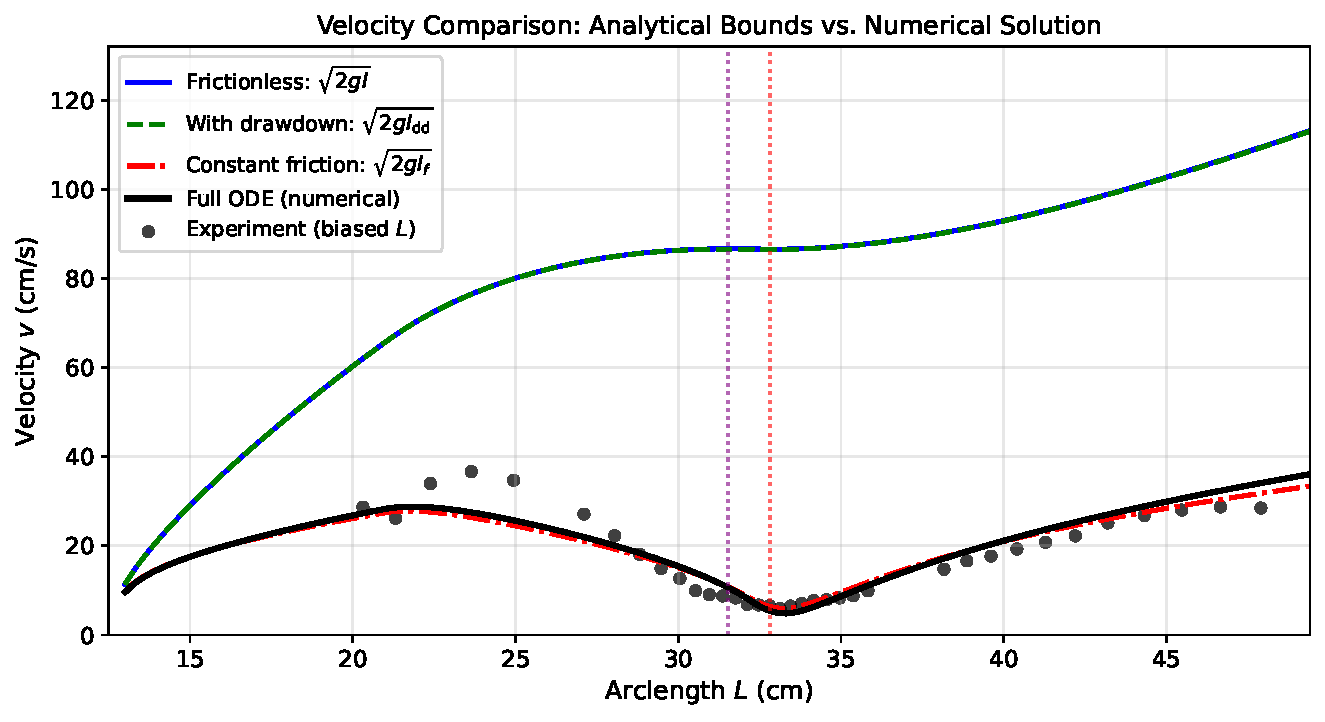
\includegraphics[width=0.9\textwidth]{figure8_velocity.pdf}
  \caption{Ταχύτητα $v(L)$ ως συνάρτηση της θέσης κατά την πλήρωση. Καμπύλες: χωρίς τριβές $\sqrt{2gI}$, με πτώση στάθμης $\sqrt{2gI_{\text{dd}}}$, σταθερή τριβή $\sqrt{2gI_f}$ και αριθμητική λύση της πλήρους Δ.Ε. Μαύρα σημεία: πειραματικές ταχύτητες ως συνάρτηση του διορθωμένου (biased) μήκους τόξου $L$. Το μοντέλο χωρίς τριβές υπερεκτιμά την ταχύτητα· το μοντέλο σταθερής τριβής είναι συντηρητικό λόγω έντονης απομείωσης της πρώιμα αποθηκευμένης ενέργειας.}
  \label{fig:velocity}
\end{figure}

% --- FIGURE 9: Time evolution ---
\begin{figure}[H]
  \centering
  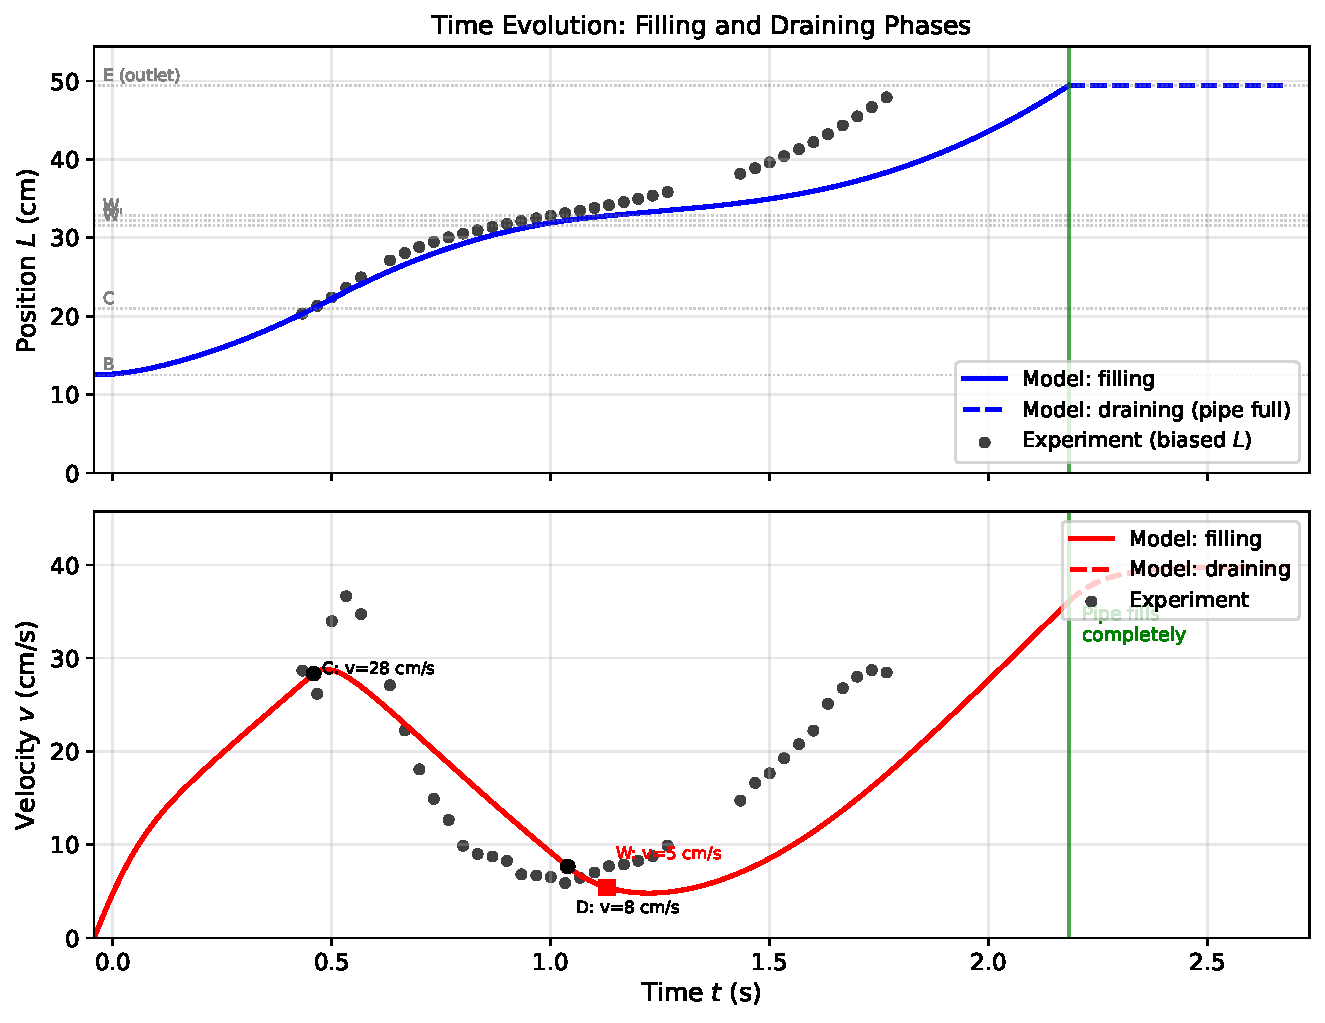
\includegraphics[width=0.9\textwidth]{figure9_time.pdf}
  \caption{Θέση $L(t)$ και ταχύτητα $v(t)$ ως συνάρτηση του χρόνου. Συνεχείς καμπύλες: αριθμητική ολοκλήρωση της πλήρους Δ.Ε. (με χρονική μετατόπιση ώστε να ευθυγραμμιστεί με το πρώτο πειραματικό σημείο). Μαύρα σημεία: πειραματικά $L_{\text{biased}}(t)$ και $v(t)$ από ανάλυση βίντεο. Σημειώνονται βασικά σημεία: $C$ (χαμηλό σημείο), $D$ (κορυφή), $W$ (τελευταία τομή με τη στάθμη), έξοδος.}
  \label{fig:time}
\end{figure}

% ══════════════════════════════════════════════════════════════════════════════
%  SECTION 8: NAVIER-STOKES DERIVATION
% ══════════════════════════════════════════════════════════════════════════════
\section{Θεμελίωση: Παραγωγή από τις Navier--Stokes}
\label{sec:navier-stokes}

Οι προηγούμενες ενότητες έχτισαν το μοντέλο μέσω φυσικής επιχειρηματολογίας. Αυτή η ενότητα το παράγει συστηματικά από τις εξισώσεις Navier--Stokes, καθιστώντας ρητή κάθε παραδοχή. Σκοπός είναι να αποσαφηνιστεί τι αποτυπώνει το μοντέλο και τι παραμελεί, συνδέοντας τη συζήτηση με τα όρια εγκυρότητας.

\subsection{Οι πλήρεις εξισώσεις}

Για ασυμπίεστο Νευτώνειο ρευστό:
\begin{align}
  \nabla \cdot \mathbf{u} &= 0, \label{eq:NS-cont} \\
  \rho\left(\frac{\partial \mathbf{u}}{\partial t} + \mathbf{u} \cdot \nabla\mathbf{u}\right) &= -\nabla p + \mu\nabla^2\mathbf{u} + \rho\mathbf{g}. \label{eq:NS-mom}
\end{align}

Αυτές ισχύουν σε κάθε σημείο. Για να καταλήξουμε σε μονοδιάστατο μοντέλο, εισάγουμε παραδοχές.

\subsection{Βήμα-βήμα απλοποίηση}

\paragraph{Παραδοχή 1: Αξονοσυμμετρική ροή σε κυκλικό σωλήνα.}
Ο σωλήνας έχει κυκλική διατομή με διάμετρο $D$. Χρησιμοποιώντας κυλινδρικές συντεταγμένες $(r, \theta, s)$ ευθυγραμμισμένες με τον άξονα του σωλήνα, η ταχύτητα είναι $\mathbf{u} = u_r\hat{r} + u_s\hat{s}$. Για λεπτούς σωλήνες ($D \ll L$), οι ακτινικές ταχύτητες είναι αμελητέες: $u_r \ll u_s$.

\emph{Τι παραμελεί:} Μη κυκλικές διατομές, τρισδιάστατα φαινόμενα στις καμπές.

\paragraph{Παραδοχή 2: Σχεδόν-μόνιμο, πλήρως ανεπτυγμένο προφίλ ταχύτητας.}
Το στιγμιαίο προφίλ ταχύτητας ταυτίζεται με το μόνιμο προφίλ για την τρέχουσα μέση ταχύτητα (παραβολικό για στρωτή ροή, λογαριθμικό για τυρβώδη).

\emph{Τι παραμελεί:} Χρόνο ανάπτυξης του προφίλ. Είναι έγκυρο όταν η ροή αλλάζει αργά σε σύγκριση με τον χρόνο ιξώδους διάχυσης $\tau_\nu = D^2/\nu$. Για $D = 5$\,mm, $\tau_\nu \approx 25$\,s· η πλήρωση συμβαίνει σε $\sim 2$\,s, άρα αυτή η παραδοχή είναι αμφίβολη κατά τη γρήγορη επιτάχυνση.

\paragraph{Παραδοχή 3: Μέσος όρος στη διατομή.}
Ορίζουμε τη μέση ταχύτητα $\bar{u}(s,t)$ ως τον μέσο όρο της $u_s$ στη διατομή. Ολοκληρώνοντας την αξονική ορμή στη διατομή:
\[
  \rho A \frac{\partial \bar{u}}{\partial t} + \rho A \bar{u}\frac{\partial \bar{u}}{\partial s} = -A\frac{\partial \bar{p}}{\partial s} + \tau_w \pi D + \rho g A \sin\theta,
\]
όπου $\tau_w = f\rho\bar{u}^2/8$ είναι η διατμητική τάση στο τοίχωμα.

\emph{Τι παραμελεί:} Ακτινικές μεταβολές πίεσης, διορθωτικούς παράγοντες ροής ορμής.

\paragraph{Παραδοχή 4: Άκαμπτο βύσμα με ομοιόμορφη ταχύτητα.}
Η ταχύτητα είναι ομοιόμορφη κατά μήκος του βύσματος: $\bar{u}(s,t) = v(t)$ για όλα τα $s$ στο βρεγμένο τμήμα. Αυτό μηδενίζει το $\partial\bar{u}/\partial s$.

\emph{Τι παραμελεί:} Συμπιεστότητα, ακουστικά κύματα, χωρικές μεταβολές ταχύτητας.

\paragraph{Παραδοχή 5: Υδροστατικές πιέσεις στα όρια.}
Στην είσοδο: $p = p_{\text{atm}} + \rho g(h_c - h_0)$. Στο μέτωπο: $p = p_{\text{atm}}$.

\emph{Τι παραμελεί:} Δυναμικές μεταβολές πίεσης στα όρια, συστολή ροής στην είσοδο.

\paragraph{Παραδοχή 6: Ασυμπίεστο ρευστό, άκαμπτα τοιχώματα σωλήνα.}
Η πυκνότητα του ρευστού $\rho$ είναι σταθερή· η διατομή του σωλήνα $A$ είναι σταθερή.

\emph{Τι παραμελεί:} Φαινόμενα συμπιεστότητας, παραμόρφωση των τοιχωμάτων υπό πίεση.

\subsection{Ολοκλήρωση κατά μήκος του βύσματος}

Ολοκληρώνοντας από την είσοδο ($s = 0$) έως το μέτωπο ($s = L$):

\paragraph{Αδράνεια:}
\[
  \int_0^L \rho A \frac{\partial v}{\partial t} ds = \rho A L \dot{v}.
\]

\paragraph{Πίεση:}
\[
  -\int_0^L A \frac{\partial \bar{p}}{\partial s} ds = A[p(0) - p(L)] = \rho g A(h_c - h_0).
\]

\paragraph{Βαρύτητα:}
\[
  \int_0^L \rho g A \sin\theta \, ds = \rho g A(h_0 - h(L)).
\]

\paragraph{Τριβές:}
\[
  \int_0^L \frac{f\rho v^2}{8}\pi D \, ds = \rho A f \frac{L}{D}\frac{v^2}{2}.
\]

Συνδυάζοντας και διαιρώντας με $\rho A L$:
\[
  \dot{v} = \frac{g}{L}[h_c - h(L)] - \frac{f}{D}\frac{v^2}{2}.
\]

Αυτό αναπαράγει την \eqref{eq:filling-ODE} χωρίς τις τοπικές απώλειες (οι οποίες απαιτούν ξεχωριστή αντιμετώπιση των τοπικών πτώσεων πίεσης).

\subsection{Σύνοψη παραδοχών}

\begin{center}
\renewcommand{\arraystretch}{1.3}
\begin{tabular}{clll}
\toprule
\# & Παραδοχή & Τι παραμελεί & Τρόπος αστοχίας \\
\midrule
1 & Αξονοσυμμετρικός, κυκλικός σωλήνας & Τρισδιάστατα φαινόμενα στις καμπές & Σφιχτές καμπές \\
2 & Σχεδόν-μόνιμο προφίλ ταχύτητας & Ανάπτυξη προφίλ & Γρήγορη επιτάχυνση \\
3 & Μέσος όρος στη διατομή & Ακτινικές μεταβολές & Μεγάλο $D/L$ \\
4 & Άκαμπτο βύσμα, ομοιόμορφη ταχύτητα & Συμπιεστότητα & Υψηλή ταχύτητα \\
5 & Υδροστατικά όρια & Δυναμικά φαινόμενα & Ταχείες ροές \\
6 & Ασυμπίεστο, άκαμπτα τοιχώματα & Συμπιεστότητα & Πολύ υψηλή πίεση \\
\bottomrule
\end{tabular}
\end{center}

% ══════════════════════════════════════════════════════════════════════════════
%  SECTION 9: VALIDITY LIMITS
% ══════════════════════════════════════════════════════════════════════════════
\section{Όρια Εγκυρότητας}
\label{sec:validity}

Κάθε μοντέλο έχει ένα πεδίο εγκυρότητας. Η κατανόηση του πού «σπάει» είναι εξίσου σημαντική με το πού λειτουργεί. Αυτή η ενότητα ποσοτικοποιεί πότε αποτυγχάνει κάθε παραδοχή.

\subsection{Επισκόπηση}

Οι παραδοχές από την \cref{sec:navier-stokes} καταρρέουν όταν:
\begin{itemize}[nosep,leftmargin=2em]
  \item Η πίεση πέσει κάτω από την πίεση ατμών $\to$ σπηλαίωση
  \item Η επιφανειακή τάση κυριαρχεί $\to$ τριχοειδικά φαινόμενα
  \item Η ροή μεταβάλλεται γρήγορα $\to$ μη μόνιμη τριβή
  \item Οι καμπές είναι σφιχτές $\to$ τρισδιάστατα φαινόμενα
\end{itemize}

Κάθε όριο χαρακτηρίζεται από μια αδιάστατη παράμετρο με κρίσιμο κατώφλι.

\subsection{Σπηλαίωση}

\subsubsection{Φυσικός μηχανισμός}

Στο υψηλότερο σημείο (κορυφή $D$), η πίεση είναι η χαμηλότερη. Αν πέσει κάτω από την πίεση ατμών $p_v \approx 2.3$\,kPa, διαλυμένα αέρια εκλύονται, σπάζοντας τη στήλη του υγρού.

\subsubsection{Ποσοτικό κριτήριο}

Χρησιμοποιώντας Bernoulli κατά μήκος του βύσματος μέχρι την κορυφή:
\[
  p_D = p_{\text{atm}} + \rho g(h_c - h_3) - \frac{1}{2}\rho v^2 - \rho g h_f.
\]

Σπηλαίωση συμβαίνει όταν $p_D < p_v$. Το μέγιστο επιτρεπτό ύψος κορυφής είναι:
\begin{equation}
  h_3 - h_c < \frac{p_{\text{atm}} - p_v}{\rho g} - \frac{v^2}{2g} - h_f \approx 10\,\text{m} - \frac{v^2}{2g} - h_f.
  \label{eq:cavitation-criterion}
\end{equation}

Για το νερό, η ατμοσφαιρική πίεση υποστηρίζει $\sim 10$\,m. Η κινητική κεφαλή και οι απώλειες τριβών μειώνουν αυτό το περιθώριο.

\subsubsection{Αξιολόγηση παραδείγματος αναφοράς}

Για ταχύτητα στην κορυφή χωρίς τριβές $v = 1.21$\,m/s και $h_3 - h_c = 4$\,cm:
\[
  p_D \approx 101300 + 1000 \times 9.81 \times (-0.04) - \frac{1}{2} \times 1000 \times 1.21^2 \approx 100200\,\text{Pa}.
\]

Αυτό είναι πολύ πάνω από $p_v = 2300$\,Pa. Περιθώριο σπηλαίωσης: $(100200 - 2300)/(1000 \times 9.81) \approx 10$\,m. Η σπηλαίωση δεν αποτελεί ανησυχία.

\subsection{Τριχοειδότητα}

\subsubsection{Φυσικός μηχανισμός}

Σε μικρές διαμέτρους, η επιφανειακή τάση επηρεάζει τη δυναμική του μετώπου. Η καμπυλότητα του μηνίσκου δημιουργεί τριχοειδική πίεση:
\[
  \Delta p_{\text{cap}} = \frac{4\gamma\cos\theta_c}{D},
\]
όπου $\theta_c$ είναι η γωνία επαφής ($\theta_c \approx 0$ για νερό σε καθαρό γυαλί/πλαστικό).

\subsubsection{Ποσοτικά κριτήρια}

Ο αριθμός Bond συγκρίνει τη βαρύτητα με την επιφανειακή τάση:
\begin{equation}
  \text{Bo} = \frac{\rho g D^2}{\gamma}.
  \label{eq:bond}
\end{equation}

Η τριχοειδότητα είναι αμελητέα όταν $\text{Bo} \gg 1$.

Ο αριθμός τριχοειδότητας συγκρίνει ιξώδεις με τριχοειδικές δυνάμεις:
\begin{equation}
  \text{Ca} = \frac{\mu v}{\gamma}.
  \label{eq:capillary}
\end{equation}

Τα δυναμικά φαινόμενα του μηνίσκου είναι αμελητέα όταν $\text{Ca} \ll 1$.

\subsubsection{Αξιολόγηση παραδείγματος αναφοράς}

Για $D = 5$\,mm:
\[
  \text{Bo} = \frac{1000 \times 9.81 \times 0.005^2}{0.073} \approx 3.4.
\]

Τριχοειδική πίεση: $\Delta p_{\text{cap}} = 4 \times 0.073/0.005 \approx 58$\,Pa, που αντιστοιχεί σε ύψος $\approx 0.6$\,cm. Αυτό είναι $\sim 40\%$ του αρχικού κινητήριου ύψους $h_c^{(0)} - h_1 = 1.5$\,cm---όχι αμελητέο για αυτή τη διάμετρο.

Στη μετρημένη μέγιστη ταχύτητα πλήρωσης $v \approx 0.36$\,m/s:
\[
  \text{Ca} = \frac{10^{-3} \times 0.36}{0.073} \approx 0.0049.
\]

Μικρό $\text{Ca}$ υποδεικνύει ότι είναι πιθανή σύζευξη ιξώδους--τριχοειδότητας στον μηνίσκο, ειδικά κοντά στην κορυφή όπου οι ταχύτητες είναι μικρές.

\paragraph{Σύσταση:} Για $D > 15$\,mm, η τριχοειδότητα είναι αμελητέα. Για $D < 5$\,mm, η τριχοειδότητα κυριαρχεί. Το παράδειγμα αναφοράς στο $D = 5$\,mm βρίσκεται κοντά στο όριο όπου η τριχοειδότητα επηρεάζει το φαινόμενο.

\subsection{Φαινόμενα εισόδου και μη μόνιμη τριβή}

\subsubsection{Φυσικός μηχανισμός}

Το μοντέλο σχεδόν-μόνιμων τριβών υποθέτει ότι το προφίλ ταχύτητας προσαρμόζεται στιγμιαία. Στην πραγματικότητα, το προφίλ αναπτύσσεται σε ένα μήκος εισόδου $L_e$, και η γρήγορη επιτάχυνση παράγει παροδικές διατμητικές τάσεις.

\subsubsection{Ποσοτικά κριτήρια}

Entrance length (turbulent):
\begin{equation}
  L_e \approx 10D \text{ to } 20D.
  \label{eq:entrance}
\end{equation}

Ο αριθμός Strouhal χαρακτηρίζει τα μη μόνιμα φαινόμενα:
\begin{equation}
  \text{St} = \frac{D}{vT},
  \label{eq:strouhal}
\end{equation}
όπου $T$ είναι ο χαρακτηριστικός χρόνος μεταβολής της ταχύτητας. Τα μη μόνιμα φαινόμενα είναι μικρά όταν $\text{St} \ll 1$.

Ο αριθμός Womersley χαρακτηρίζει ταλαντωτικές ροές:
\begin{equation}
  \text{Wo} = D\sqrt{\frac{\omega}{\nu}},
  \label{eq:womersley}
\end{equation}
όπου $\omega$ είναι η γωνιακή συχνότητα. Για την πλήρωση, $\omega \sim 1/T$.

\subsubsection{Αξιολόγηση παραδείγματος αναφοράς}

Για το παράδειγμα αναφοράς, η ροή είναι κυρίως στρωτή ($\text{Re} \lesssim 2000$). Το μήκος εισόδου στη στρωτή ροή κλιμακώνεται ως $L_e/D \approx 0.05\,\text{Re}$, οπότε για $\text{Re} \approx 1800$:
\[
  \frac{L_e}{D} \approx 90 \quad \Rightarrow \quad L_e \approx 90 \times 0.5\,\text{cm} \approx 45\,\text{cm}.
\]
Τα τμήματα έχουν μήκος 8--17\,cm, άρα η ροή πιθανότατα αναπτύσσεται σε μεγάλο μέρος του σωλήνα· αυτό είναι μια εύλογη πηγή απόκλισης από τις παραδοχές σχεδόν-μόνιμων τριβών.

Για $v \approx 0.36$\,m/s που μεταβάλλεται σε χρόνο $T = 0.5$\,s:
\[
  \text{St} = \frac{0.005}{0.36 \times 0.5} \approx 0.028.
\]

Μικρός αριθμός Strouhal υποδηλώνει ότι τα μη μόνιμα φαινόμενα είναι μέτρια, αλλά μπορεί να έχουν σημασία κατά την αρχική επιτάχυνση και κοντά στην κορυφή όπου οι ταχύτητες είναι χαμηλές.

\subsection{Τρισδιάστατα φαινόμενα στις καμπές}

\subsubsection{Φυσικός μηχανισμός}

Η ροή μέσα από καμπές δημιουργεί δευτερογενείς ροές (στροβίλους Dean) που ενισχύουν την ανάμιξη και τη διάχυση. Οι συντελεστές τοπικών απωλειών $K$ αποτυπώνουν εμπειρικά αυτά τα φαινόμενα.

\subsubsection{Ποσοτικό κριτήριο}

Ο αριθμός Dean χαρακτηρίζει την ένταση των δευτερογενών ροών:
\begin{equation}
  \text{De} = \text{Re}\sqrt{\frac{D}{2R}},
  \label{eq:dean}
\end{equation}
όπου $R$ είναι η ακτίνα καμπυλότητας της καμπής. Οι δευτερογενείς ροές είναι σημαντικές όταν $\text{De} > 100$.

\subsubsection{Αξιολόγηση παραδείγματος αναφοράς}

Για σφιχτές καμπές $180^\circ$ με $R \approx 2D$ και $\text{Re} \approx 1800$:
\[
  \text{De} \approx 1800 \times \sqrt{\frac{1}{4}} \approx 900.
\]

Αυτός ο αριθμός Dean υποδεικνύει ισχυρές δευτερογενείς ροές. Στην πράξη, τα φαινόμενα εισόδου/εξόδου και οι απώλειες καμπών μπορούν να ενσωματωθούν σε ένα αποτελεσματικό $\sum K$ όταν η λεπτομερής γεωμετρία των καμπών δεν χαρακτηρίζεται· στο παράδειγμα αναφοράς, η προσαρμογή στη μετρημένη $v(L)$ δίνει $\sum K \approx 14.4$ (τάξης $3$--$4$ ανά καμπή για τέσσερις καμπές).

\subsection{Διαγράμματα περιοχών εγκυρότητας}

Ο \Cref{fig:validity} παρουσιάζει τα όρια εγκυρότητας σε τρεις χώρους παραμέτρων.

% --- FIGURE 10: Validity regime diagrams ---
\begin{figure}[H]
  \centering
  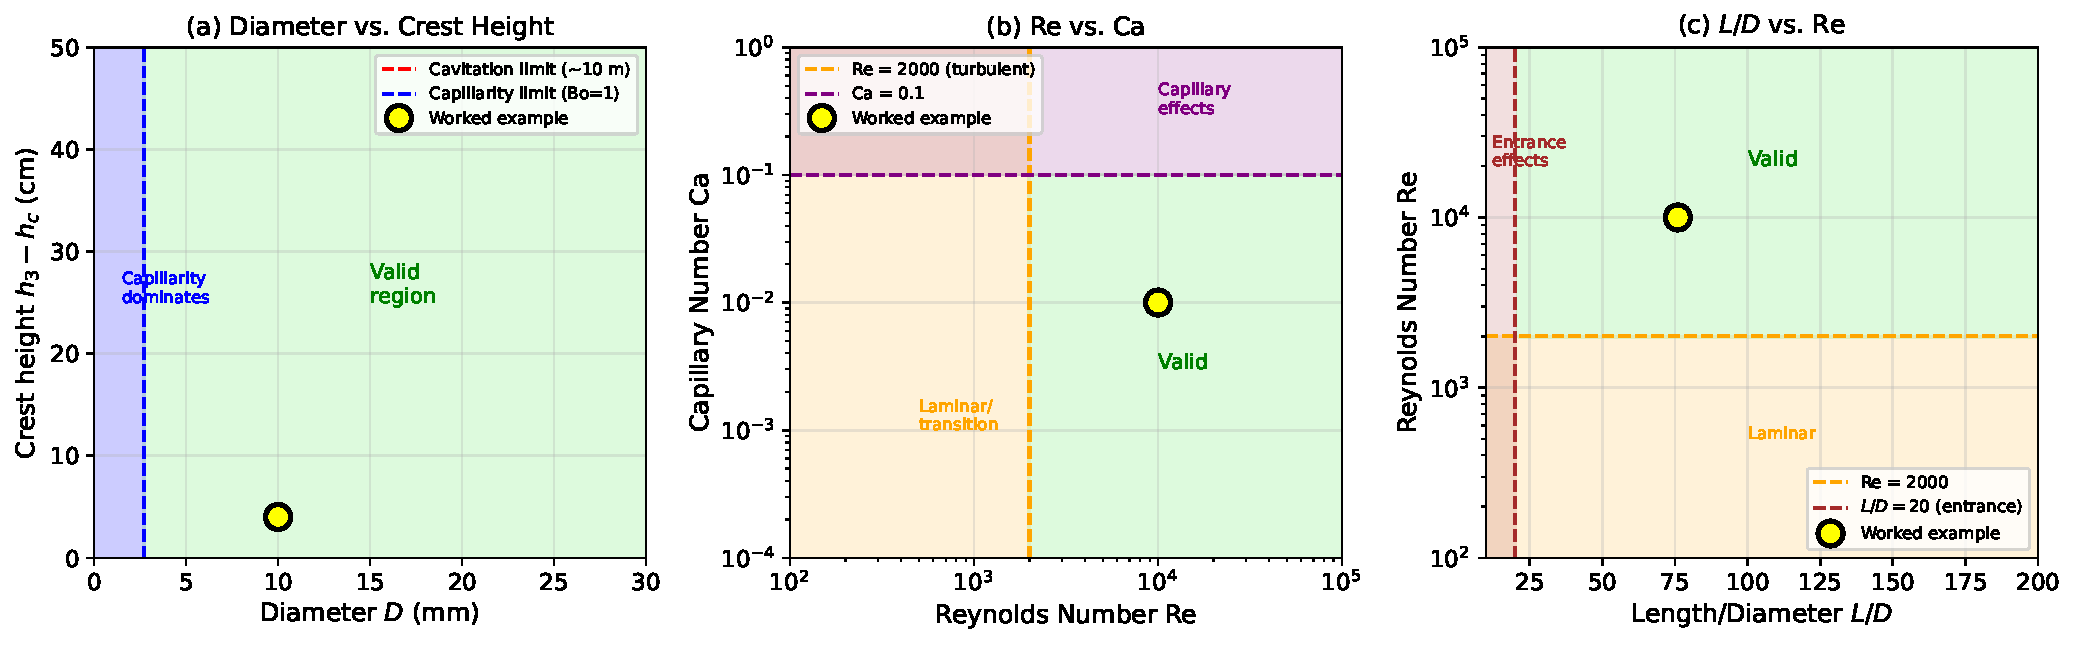
\includegraphics[width=0.95\textwidth]{figure10_validity.pdf}
  \caption{Διαγράμματα περιοχών εγκυρότητας. (a) Διάμετρος $D$ ως συνάρτηση του ύψους κορυφής $h_3 - h_c$: η σπηλαίωση περιορίζει ψηλές κορυφές· η τριχοειδότητα περιορίζει μικρές διαμέτρους. (b) Αριθμός Reynolds ως συνάρτηση του αριθμού τριχοειδότητας: αναδεικνύει το όριο στρωτής/μεταβατικής ροής και το καθεστώς μικρού $\text{Ca}$. (c) $L/D$ ως συνάρτηση του Reynolds: μεγάλος $L/D$ σημαίνει ροή που κυριαρχείται από τριβές· οι παραδοχές μήκους εισόδου και σχεδόν-μόνιμων τριβών γίνονται αμφίβολες σε χαμηλά Re. Το παράδειγμα αναφοράς (σημειωμένο) βρίσκεται κοντά στα όρια τριχοειδότητας/φαινομένων εισόδου.}
  \label{fig:validity}
\end{figure}

\subsubsection{Διάγραμμα (a): $D$ ως συνάρτηση του $h_3 - h_c$}

Άνω όριο: όριο σπηλαίωσης, $(h_3 - h_c) < 10\,\text{m} - v^2/2g$. Κάτω όριο για μικρό $D$: η τριχοειδότητα κυριαρχεί όταν $\text{Bo} < 1$, δηλαδή $D < \sqrt{\gamma/\rho g} \approx 2.7$\,mm.

\emph{Ερμηνεία:} Το παράδειγμα αναφοράς ($D = 5$\,mm, $h_3 - h_c = 0.5$\,cm) είναι μακριά από τη σπηλαίωση αλλά κοντά στο καθεστώς όπου η τριχοειδότητα επηρεάζει το φαινόμενο.

\subsubsection{Διάγραμμα (b): Re ως συνάρτηση του Ca}

Έγκυρη περιοχή: $\text{Ca} < 0.1$ (μικρή επίδραση τριχοειδικών φαινομένων στον μηνίσκο) και αρκετά υψηλό Re ώστε να ισχύουν οι παραδοχές σχεδόν-μόνιμης/πλήρως ανεπτυγμένης ροής. Το παράδειγμα αναφοράς λειτουργεί σε $\text{Re} \sim 10^3$, $\text{Ca} \sim 5\times 10^{-3}$: ο Ca είναι μικρός, αλλά το Re είναι κοντά στο όριο στρωτής/μεταβατικής ροής, άρα τα φαινόμενα αναπτυσσόμενης ροής μπορεί να έχουν σημασία.

\emph{Ερμηνεία:} Η μείωση της διαμέτρου ωθεί προς υψηλότερο Re (για σταθερή ταχύτητα) αλλά και προς μεγαλύτερη τριχοειδική επίδραση. Υπάρχει ένα βέλτιστο εύρος διαμέτρων.

\subsubsection{Διάγραμμα (c): $L/D$ ως συνάρτηση του Re}

Για σχεδόν-μόνιμες τριβές, κάθε τμήμα θα πρέπει να υπερβαίνει το μήκος εισόδου. Χρησιμοποιώντας την τυρβώδη εκτίμηση $L_e \approx 10D$ έως $20D$, το παράδειγμα αναφοράς έχει $L_i/D \approx 17$ έως 34 και θα ήταν οριακό. Στο στρωτό καθεστώς, όμως, τα μήκη εισόδου μπορούν να είναι πολύ μεγαλύτερα ($L_e/D \sim 0.05\,\text{Re}$), οπότε αυτό είναι ένας βασικός περιορισμός.

\emph{Ερμηνεία:} Συντομότερα τμήματα ή μικρότερες διάμετροι ωθούν προς το καθεστώς όπου κυριαρχούν τα φαινόμενα εισόδου και το μοντέλο τριβών χάνει ακρίβεια.

\subsubsection{Σύνοψη}

Το παράδειγμα αναφοράς βρίσκεται κοντά στα όρια τριχοειδότητας και φαινομένων εισόδου. Αυτό υποδηλώνει ότι αποκλίσεις μεταξύ του απλούστερου μονοδιάστατου μοντέλου και του πειράματος μπορεί να οφείλονται στη φυσική του μηνίσκου και σε αναπτυσσόμενες/μη μόνιμες τριβές, και όχι μόνο στη γεωμετρία.

% ══════════════════════════════════════════════════════════════════════════════
%  SECTION 10: CONCLUSION
% ══════════════════════════════════════════════════════════════════════════════
\section{Συμπεράσματα}
\label{sec:conclusion}

Η εργασία αυτή ανέπτυξε ένα θεωρητικό πλαίσιο για τη διερεύνηση αυτοεκκινούμενων σιφώνων μέσω στρωματωτής ανάλυσης.

Το μοντέλο χωρίς τριβές απομονώνει τη γεωμετρία ως καθοριστική παράμετρο. Το ενεργειακό ολοκλήρωμα $I(L)$ αθροίζει συνεισφορές στην κινητική ενέργεια, σταθμισμένες με $1/L$ ώστε να ληφθεί υπόψη η αυξανόμενη μάζα του βύσματος. Το κριτήριο προπλήρωσης $I(S_W) > 0$ υπολογίζεται σε κλειστή μορφή για κατά τμήματα γραμμικές γεωμετρίες.

Η προσθήκη πτώσης στάθμης εισάγει τον λόγο εμβαδών $A/A_0$. Το τροποποιημένο ολοκλήρωμα $I_{\text{dd}}(L)$ παραμένει αναλυτικό. Για μεγάλα δοχεία ($A/A_0 < 0.01$), η πτώση στάθμης είναι αμελητέα.

Η προσθήκη τριβών εισάγει το $\varepsilon/D$ και τους συντελεστές απωλειών καμπών $K$. Το ολοκλήρωμα σταθερής τριβής $I_f(L)$ δείχνει πώς η διάχυση απομειώνει την ενέργεια που έχει «αποθηκευτεί» νωρίς μέσω ενός εκθετικού παράγοντα. Αυτό το ενδιάμεσο μοντέλο δίνει συντηρητικές εκτιμήσεις ταχύτητας.

Η σύγκριση των τριών ολοκληρωμάτων στο ίδιο γράφημα οπτικοποιεί το ενεργειακό κόστος κάθε επίδρασης. Για το παράδειγμα αναφοράς με αποτελεσματικό $\sum K \approx 14.4$, το μοντέλο σταθερής τριβής προβλέπει ότι οι τριβές κυριαρχούν, μειώνοντας την ενέργεια κατά $\sim 99.5\%$· η πτώση στάθμης συμβάλλει μόνο κατά $\sim 0.1\%$. Αυτή η ευαισθησία στις τοπικές απώλειες αναδεικνύει τη σημασία της γεωμετρίας των καμπών: μεγαλύτερο $\sum K$ θα μείωνε πολύ πιο έντονα τη διαθέσιμη ενέργεια.

Η πλήρης δυναμική απαιτεί αριθμητική ολοκλήρωση λόγω της τριβής που εξαρτάται από την ταχύτητα, όμως τα αναλυτικά ολοκληρώματα περικλείουν τη λύση. Η φάση εκκένωσης, που κυριαρχεί στον συνολικό χρόνο σιφωνισμού, περιγράφεται από μια απλούστερη Δ.Ε. όπου το μήκος του βύσματος είναι σταθερό.

Η παραγωγή από τις Navier--Stokes καθιστά ρητή κάθε παραδοχή και συνδέει τη συζήτηση με τα όρια εγκυρότητας. Η σπηλαίωση, η τριχοειδότητα, τα φαινόμενα εισόδου και οι τρισδιάστατες ροές στις καμπές έχουν χαρακτηριστικές αδιάστατες παραμέτρους. Τα διαγράμματα περιοχών δείχνουν πού το μοντέλο είναι αξιόπιστο και πού μπορεί να αποτύχει.

Το πλαίσιο επιτρέπει συστηματική διερεύνηση παραμέτρων:
\begin{itemize}[nosep,leftmargin=2em]
  \item \textbf{Η γεωμετρία} καθορίζει το ενεργειακό ισοζύγιο χωρίς τριβές---τον θεμελιώδη παράγοντα της προπλήρωσης.
  \item \textbf{Οι ιδιότητες του σωλήνα} ($D$, $\varepsilon/D$, $K$) καθορίζουν τις απώλειες τριβών.
  \item \textbf{Το μέγεθος του συστήματος} ($A/A_0$) καθορίζει την πτώση στάθμης.
  \item \textbf{Οι βέλτιστες διατάξεις ελαχιστοποιούν τις απώλειες καμπών.} Μόλις η γεωμετρία εξασφαλίσει $I(S_W) > 0$, η μείωση των συντελεστών τοπικών απωλειών (μείωση του $\sum K$ με ομαλές, ήπιες καμπές) είναι συνήθως ο πιο αποτελεσματικός τρόπος για να αυξηθεί το περιθώριο προπλήρωσης και να μειωθεί ο χρόνος πλήρωσης.
\end{itemize}

Αλλαγές που βελτιώνουν την προπλήρωση συνήθως επιταχύνουν και την πλήρωση: πιο απότομες πτώσεις, χαμηλότερες κορυφές, μεγαλύτερες διάμετροι, πιο λείοι σωλήνες. Εξαίρεση αποτελεί το μέγεθος του δοχείου: μεγαλύτερα δοχεία διευκολύνουν την προπλήρωση αλλά αυξάνουν τον χρόνο εκκένωσης.

Το μοντέλο παρέχει αναλυτική κατανόηση για το πώς κάθε παράμετρος επηρεάζει τη διαδικασία του σιφωνισμού---μια κατανόηση που η αριθμητική προσομοίωση από μόνη της δεν μπορεί να προσφέρει.

% ══════════════════════════════════════════════════════════════════════════════
%  APPENDIX: FRICTION CORRELATIONS
% ══════════════════════════════════════════════════════════════════════════════
\appendix
\section{Συσχετίσεις Τριβών}
\label{app:friction}

\subsection{Η συσχέτιση Churchill}

Η συσχέτιση Churchill (1977) παρέχει έναν ενιαίο τύπο για τον συντελεστή τριβής Darcy, έγκυρο σε όλα τα καθεστώτα ροής:
\begin{equation}
  f = 8\left[\left(\frac{8}{\text{Re}}\right)^{12} + \frac{1}{(A_C + B_C)^{3/2}}\right]^{1/12},
  \label{eq:churchill-full}
\end{equation}
όπου
\begin{align}
  A_C &= \left[2.457\ln\left(\frac{1}{(7/\text{Re})^{0.9} + 0.27(\varepsilon/D)}\right)\right]^{16}, \\
  B_C &= \left(\frac{37530}{\text{Re}}\right)^{16}.
\end{align}

\subsection{Οριακή συμπεριφορά}

\paragraph{Στρωτό όριο ($\text{Re} \to 0$):}
Ο πρώτος όρος $(8/\text{Re})^{12}$ κυριαρχεί. Αναπτύσσοντας:
\[
  f \to 8 \times \frac{8}{\text{Re}} = \frac{64}{\text{Re}},
\]
δηλαδή το ακριβές αποτέλεσμα Hagen--Poiseuille.

\paragraph{Τυρβώδες όριο ($\text{Re} \to \infty$):}
Ο δεύτερος όρος κυριαρχεί. Καθώς $B_C \to 0$, $f \to 8/(A_C)^{1/8}$, που αναπαράγει την εξίσωση Colebrook--White:
\[
  \frac{1}{\sqrt{f}} = -2\log\left(\frac{\varepsilon/D}{3.7} + \frac{2.51}{\text{Re}\sqrt{f}}\right).
\]

\paragraph{Μεταβατική περιοχή:}
Και οι δύο όροι συνεισφέρουν, παρέχοντας ομαλή παρεμβολή. Το προκύπτον $f$ είναι συνεχές και παραγωγίσιμο.

\subsection{Σύγκριση με Colebrook--White}

Η εξίσωση Colebrook--White είναι μη ρητή και απαιτεί επαναληπτική λύση. Ρητές προσεγγίσεις (Haaland, Swamee--Jain) εισάγουν σφάλμα 1--2\%. Η Churchill ταιριάζει με Colebrook--White στο τυρβώδες καθεστώς με απόκλιση έως 1\%, ενώ καλύπτει και τη στρωτή ροή.

Για την πλήρωση του σιφώνα όπου το Re κυμαίνεται από 0 έως $\sim 10^4$, η Churchill είναι η φυσική επιλογή: δεν απαιτεί λογική αλλαγής καθεστώτων και χειρίζεται όλο το εύρος με συνέπεια.

\subsection{Ζητήματα ακρίβειας}

Η Colebrook--White είναι εμπειρική προσαρμογή στα πειράματα του Nikuradse τη δεκαετία του 1930, με ακρίβεια $\pm 5$--$10\%$. Η αβεβαιότητα στον συντελεστή τριβής είναι συγκρίσιμη με τις αβεβαιότητες στους συντελεστές τοπικών απωλειών και στην παραδοχή σχεδόν-μόνιμης ροής. Για διερεύνηση παραμέτρων, η συσχέτιση Churchill είναι υπεραρκετή.

% --- FIGURE A1: Friction correlation comparison ---
\begin{figure}[H]
  \centering
  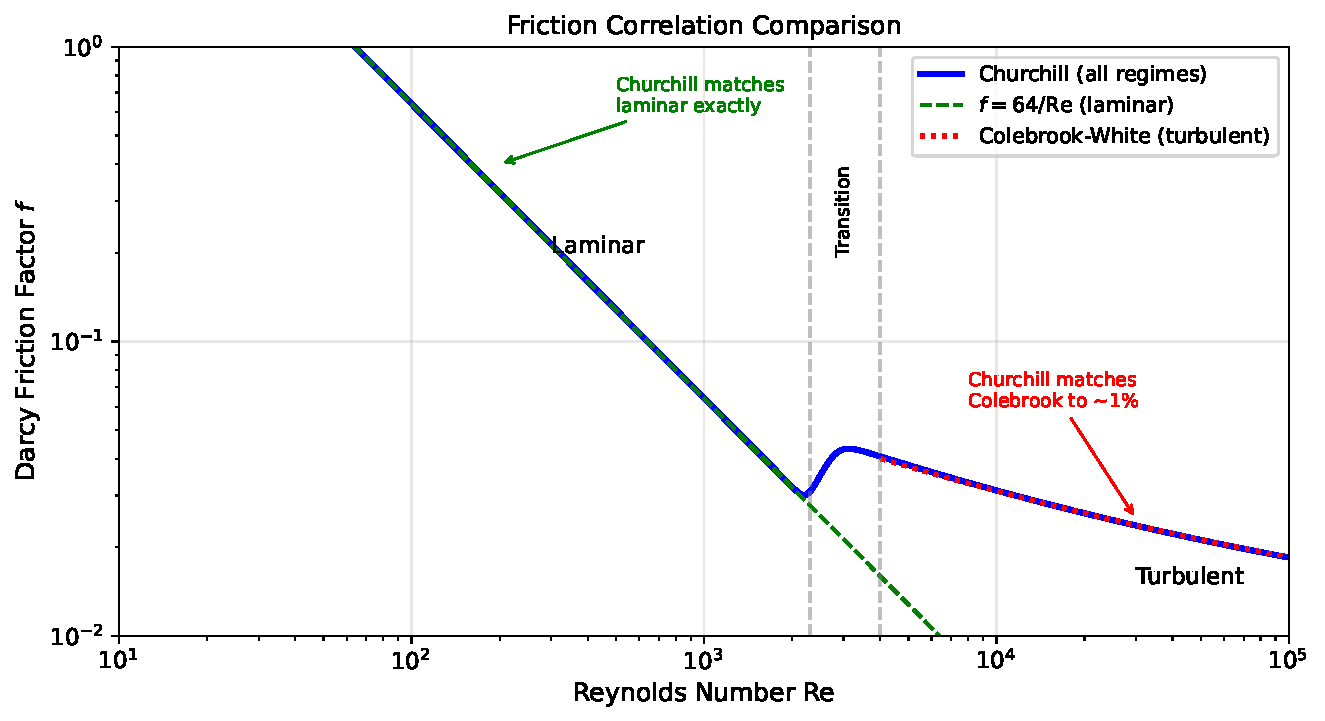
\includegraphics[width=0.9\textwidth]{figureA1_friction_comparison.pdf}
  \caption{Σύγκριση συσχετίσεων τριβών. Συνεχής: Churchill. Διακεκομμένη: Colebrook--White (μόνο τυρβώδες). Διάστικτη: $f = 64/\text{Re}$ (στρωτό). Η Churchill γεφυρώνει ομαλά όλα τα καθεστώτα. Για $\text{Re} > 4000$, ταιριάζει με Colebrook--White με απόκλιση έως 1\%.}
  \label{fig:friction-comparison}
\end{figure}

\end{document}
